\documentclass[letterpaper]{article}

\usepackage{natbib,alifeconf}  %% The order is important

\usepackage{hyperref}

\usepackage{subcaption}

\usepackage{hhline}

\usepackage{filecontents}
\usepackage{csvsimple}

\usepackage{amsmath}


\ifdefined\mydraft
\mydraft
\fi

\graphicspath{{img/}}

% *****************
%  Requirements:
% *****************
%
% - All pages sized consistently at 8.5 x 11 inches (US letter size).
% - PDF length <= 8 pages for full papers, <=2 pages for extended
%    abstracts.
% - Abstract length <= 250 words.
% - No visible crop marks.
% - Images at no greater than 300 dpi, scaled at 100%.
% - Embedded open type fonts only.
% - All layers flattened.
% - No attachments.
% - All desired links active in the files.

% Note that the PDF file must not exceed 5 MB if it is to be indexed
% by Google Scholar. Additional information about Google Scholar
% can be found here:
% http://www.google.com/intl/en/scholar/inclusion.html.


% If your system does not generate letter format documents by default,
% you can use the following workflow:
% latex example
% bibtex example
% latex example ; latex example
% dvips -o example.ps -t letterSize example.dvi
% ps2pdf example.ps example.pdf


% For pdflatex users:
% The alifeconf style file loads the "graphicx" package, and
% this may lead some users of pdflatex to experience problems.
% These can be fixed by editing the alifeconf.sty file to specify:
% \usepackage[pdftex]{graphicx}
%   instead of
% \usepackage{graphicx}.
% The PDF output generated by pdflatex should match the required
% specifications and obviously the dvips and ps2pdf steps become
% unnecessary.


% Note:  Some laser printers have a serious problem printing TeX
% output. The use of ps type I fonts should avoid this problem.


\title{TODO SignalGP Dishtiny}
\author{Matthew Andres Moreno$^{1}$ \and Charles Ofria$^{1}$ \\
\mbox{}\\
$^1$BEACON Center, Michigan State University, East Lansing, MI 48824 \\
mmore500@msu.edu} % email of corresponding author

% For several authors from the same institution use the same number to
% refer to one address.
%
% If the names do not fit well on one line use
%         Author 1, Author 2 ... \\ {\Large\bf Author n} ...\\ ...
%
% If the title and author information do not fit in the area
% allocated, place \setlength\titlebox{<new height>} after the
% \documentclass line where <new height> is 2.25in



\begin{document}
\maketitle

\begin{abstract}

Evolutionary transitions in individuality have profoundly shaped natural evolutionary history.
These transitions include episodes where independent replicating entities united to form more complex replicating entities.
If the derived replicating entity is composed of lower-level replicating entity kin, then such a transition is termed fraternal.
Examples of fraternal transitions include the evolution of multicellularity and the evolution of eusocial insect colonies.
The conditions necessary for fraternal transitions to arise and the mechanisms by which such transitions take place continue to be fruitful targets of scientific interest.
We work with replicators controlled by heritable open-ended event-driven computer programs.
Replicators were allowed to unite into explicitly registered kin cooperating groups.
We observe cells evolve phenotypes characteristic of fraternal transitions in individuality with respect to these cooperating groups: reproductive division of labor, resource sharing (including, in some treatments, endowment of offspring propagule groups), asymmetrical within-group and inter-group phenomena mediated by cell-cell messaging, morphological patterning, gene-regulation mediated life cycles, and adaptive apoptosis.
From an applied perspective, fraternal transitions in individuality might yield digital organisms that exhibit more sophisticated, and potentially useful, capabilities.
As an experimental system, open-ended digital multicellular systems allow pursuit of biologically-motivated questions that otherwise, \textit{in vivo}, might require experiments that are slow, expensive, or call for physically impracticable manipulations.

\end{abstract}


\section{Introduction}

It is the aim of Artificial Life research to realize engineered systems that exhibit properties of biological life in order to study them, but also with an eye towards applications such as artificial intelligence \citep{bedau2003artificial}.
Studies of evolution have been of particular interest to the community, especially in regard to how organisms are produced with increasing sophistication and complexity \citep{goldsby2017increasing}.
This particular issue is often described as ``open-ended evolution.''
Although precise definitions and measures of open-ended evolution are still being established, this term is generally understood to refer to evolving systems that exhibit the continued production of novelty \citep{taylor2016open}.
Evolutionary transitions in individuality, which are key to the complexification and diversification of biological life \citep{smith1997major}, have been highlighted as key research targets with respect to the question of open-ended evolution \citep{ray1996evolving, banzhaf2016defining}.
In an evolutionary transition of individuality, a new, more complex replicating entity is derived from the combination of cooperating replicating entities which have entwined their long-term fates \citep{west2015major}.
Eusocial insect colonies and multicellular organisms exemplify this phenomenon \citep{smith1997major}.
Like the definition of open-ended evolution, the notion of what constitutes an evolutionary individual is not concretely established;
close coordination and cooperation between component entities, reproductive division of labor between component entities, reproductive bottlenecks of component entities, reproductive lineages (e.g. parent-offspring relationships) at the level of the ensemble are among criteria cited for evolutionary individuality
\citep{ereshefsky2015rethinking, bouchard2013symbiotic}.

In order to study evolutionary transitions of individuality, we must devise a system in which we expect such transitions to occur in a detectable manner.
To this end, we introduce the DISHTINY (DIStributed Hierarchical Transitions of IndividualitY) platform, which seeks to achieve this goal by explicitly registering organisms in cooperating groups that coordinate spatiotemporally to maximize the harvest of a resource.
Detection of a transition of individuality in DISHTINY is accomplished by identifying resource-sharing and reproductive division of labor among organisms registered to the same cooperating group.
Our system is designed such that hierarchal transitions across an arbitrary number of levels of individuality can be selected for and detected.
We have focused this system on a rigid form of major transition using simple organisms, but the underlying principles that we are studying here can be applied to a wide range of artificial life systems.
Furthermore, DISHTINY is decentralized;
it is amenable to massive parallelization via distributed computing.
We believe that such scalability --- with respect to both concept and implementation --- is an essential consideration in the pursuit of artificial systems capable of generating complexity and novelty rivaling that of biological life via open-ended evolution.

%@CAO, I'm cutting these for now to save space.
%We begin by laying out the design of the DISHTINY platform.
%Then, we introduce a model organism used to test for selection for high-level individuality in DISHTINY.
%Finally, we discuss the results of ecological competition and evolutionary experiments, which demonstrate selection for --- and emergence of --- high-level individuality in DISHTINY.


\section{Methods}

We manually designed strategies that organisms could use to cooperate to experimentally demonstrate that the DISHTINY platform selects for detectable hierarchical transitions of individuality.

\subsection{DISHTINY}

\begin{figure*}[t]
\begin{center}
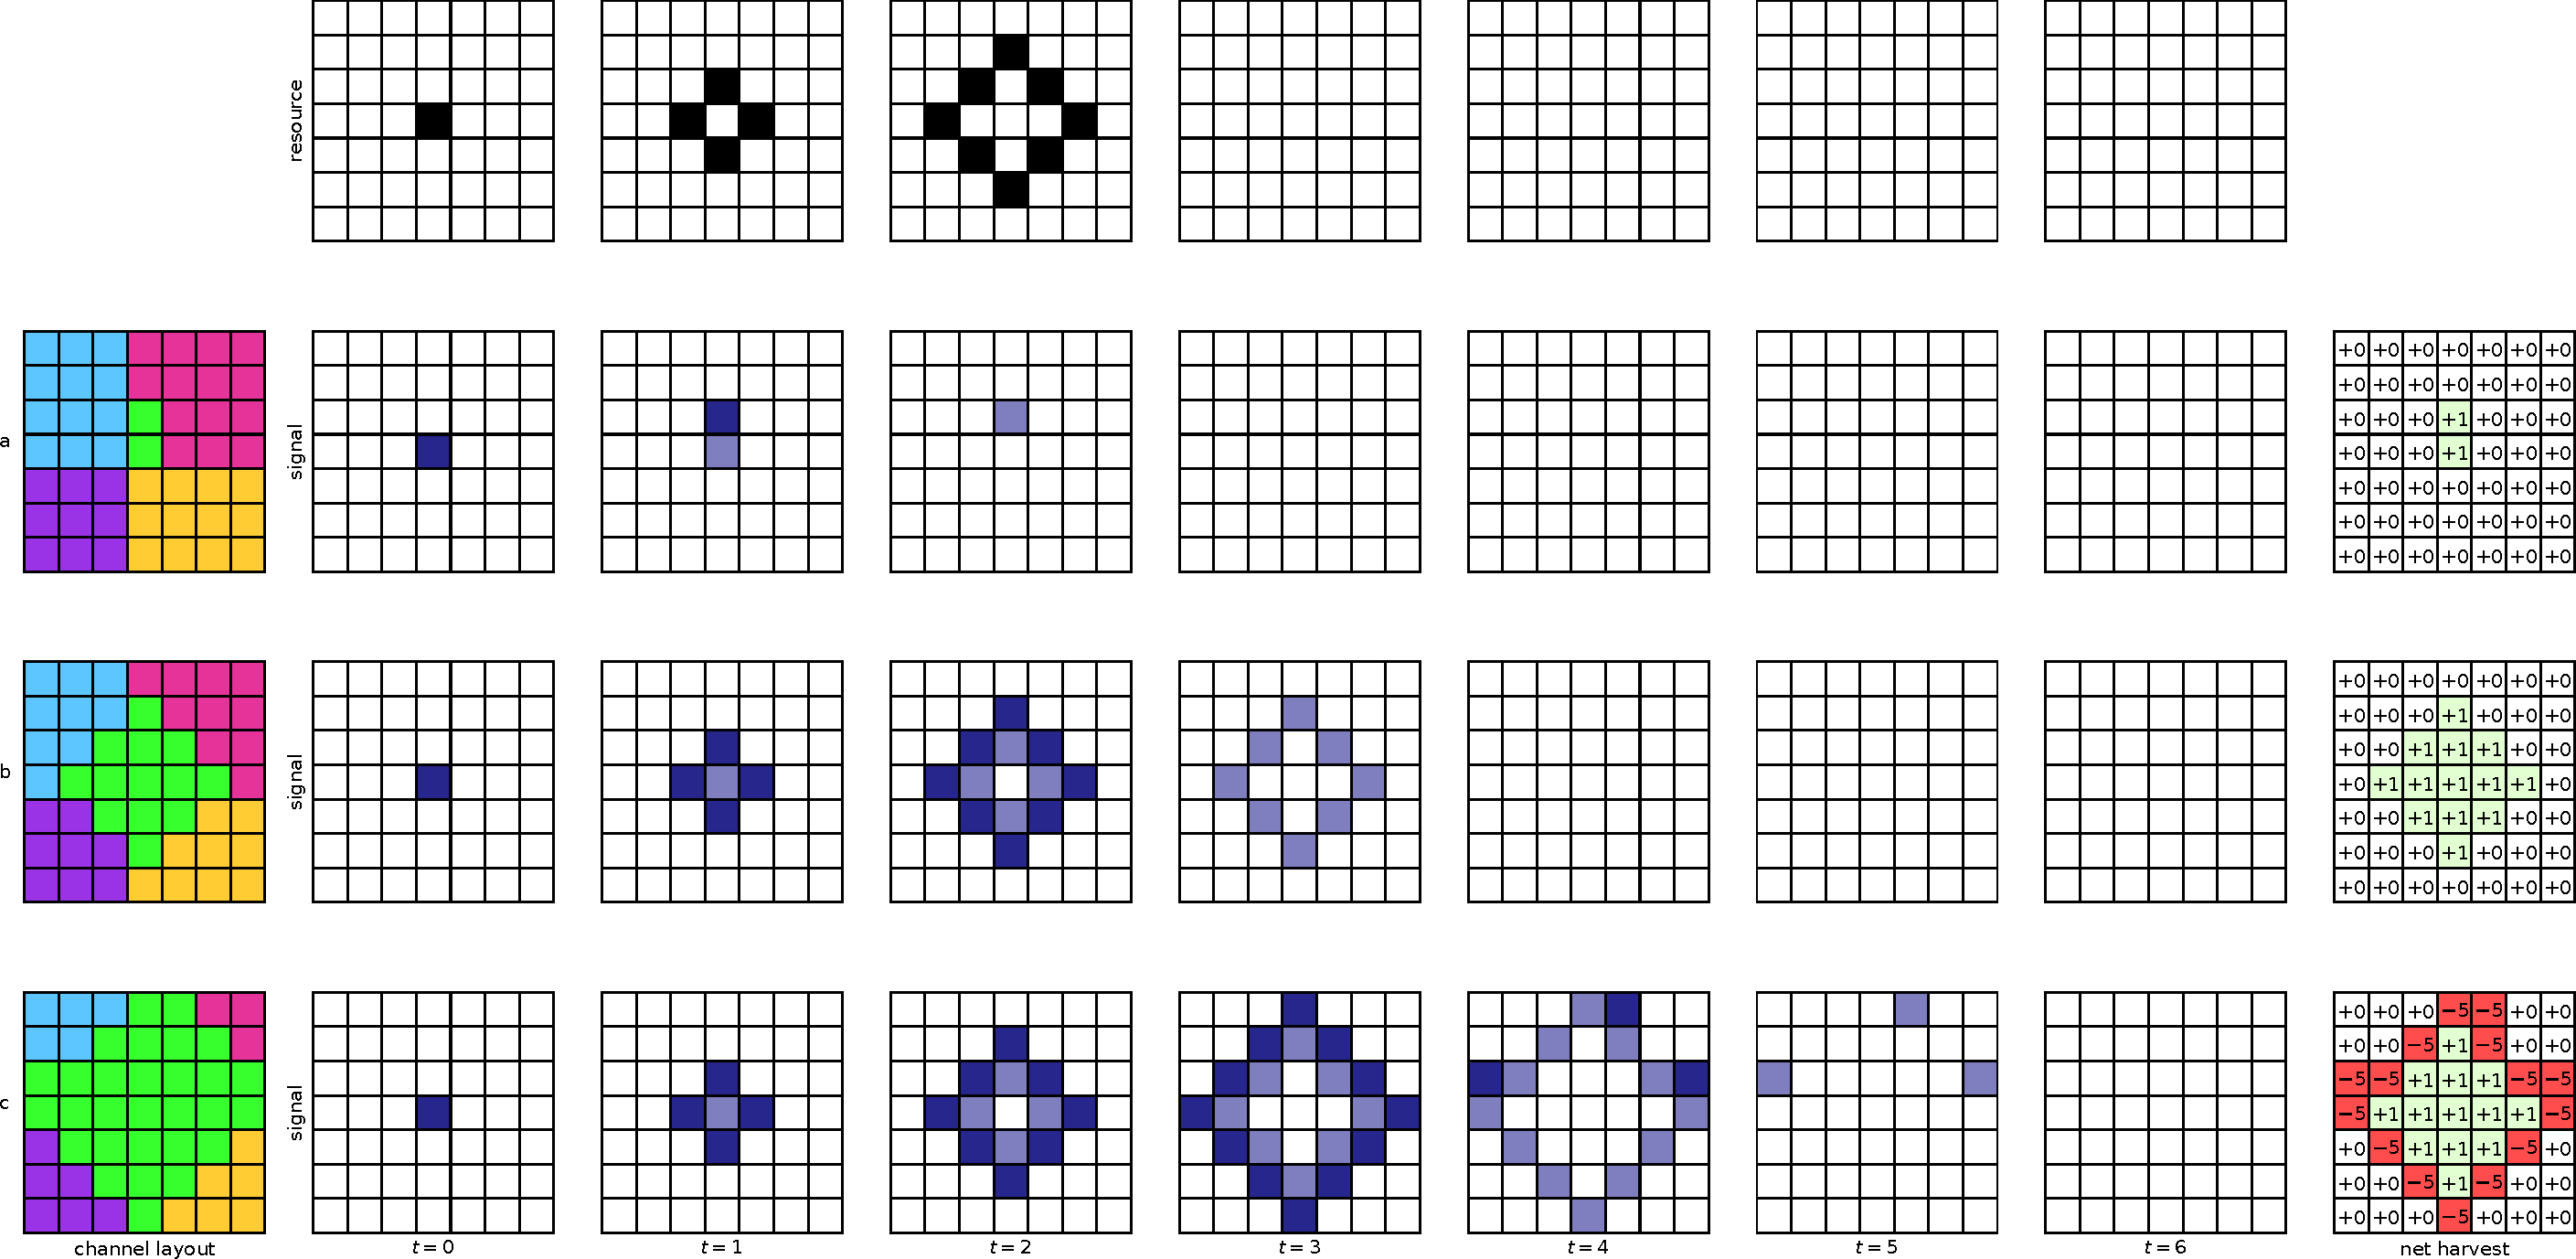
\includegraphics[width=2.0\columnwidth]{img/explanatory}
\caption{Activation-quiescence signaling, and net resource collection for three different channel configurations during a single resource wave events.}
\label{fig:explanatory}
\end{center}
\end{figure*}


We will begin by discussing the implementation of our artificial environment at a single hierarchical level, then lay out how the system scales to multiple levels.

A single continuous-valued resource is tracked.
When organisms accrue sufficient resource, they may choose to pay a cost of $-8$ to reproduce.
As shown Figure \ref{fig:explanatory}, resource is distributed in waves that emanate from a single point.
With each simulation update, the resource wave advances one grid tile outward until it reaches a predefined extent.
The resource wave then ceases.
Coincident with the inception of each resource wave, an activation-quiescence signal wave is triggered at the wave's center point.
Example signal waves are shown in Figure \ref{fig:explanatory}.
With every update, the signal wave passes to adjoining cells registered to the same channel as the cell it emanates from.
The signal wave is not propagated to any cells on any other channel.
In this way, cells sharing the channel of the cell where the resource wave originated are activated coincident with the resource wave.

In order to obtain resource, a cell must be activated by a signal wave as the resource wave passes over.
The cell at the center of a resource wave will always be activated and absorb resource.
However, immediately adjacent cells can only obtain resource by the action of the signal wave --- by sharing the channel of the originating cell.
Cells further off depend on a continuous path of cells extending from the originating cell that signal on the originating channel in order to obtain resource.
As shown in Example $a$ of Figure \ref{fig:explanatory}, the rate of resource collection is determined by the size of a channel signaling network; small or fragmented channel networks will tend to frequently miss out on resource as it passes over.

Importantly, a significant activation cost is paid by each cell that is activated by a signal wave.
This activation cost is outweighed by the amount of resource collected --- cells that activate in concert with a resource wave take away a net benefit.
Recall, though, that resource waves have a limited extent.
Cells that activate outside of the extent of the resource wave or activate out of sync with the resource wave (i.e. are not connected via a direct path to the originating cell) pay a cost.
Cells that frequently activate erroneously bankrupt and die.
In our implementation, organisms that accrue a resource debt of $-11$ or greater are killed.
This scenario is depicted in Example $c$ of Figure \ref{fig:explanatory}.

In this manner, ``Goldilocks'' --- not to small and not too big --- same-channel signaling networks are selected for.
In our implementation, resource waves are seeded at a single location drawn  with uniform probability from the toroidal grid.
Based on this location, resource wave seeds are tiled over the toroidal grid so as to have kissing --- but not overlapping --- extents.
All the waves are updated to completion in synchrony.
Then, another batch of resource waves is seeded.
This process ensures that selection for ``Goldilocks'' same-channel signaling networks is uniformly distributed over the toroidal grid.

Organisms may control the size and shape of their same-channel signaling group by strategic control of reproduction.
Three choices are afforded: whether to reproduce at all, where among the four adjoining tiles of the toroidal grid to place their offspring, and whether the offspring should be registered to the parent's signaling channel or should instead be registered to a randomly chosen signaling channel.
New channels IDs are drawn uniformly from the integer range 1-4194303.
No guarantees are made about the uniqueness of an offspring's channel ID with respect to the channel IDs of the parent or other neighboring cells.

Hierarchical levels are introduced into the system through multiple instantiations of this resource wave/channel-signaling wave scheme.
In our experiments, we worked with two resource wave/channel-signaling levels.
We refer to them as level zero and level one.
On the zero level, resource waves extended a radius of four toroidal tiles, granted a resource value of $+6$, and cost a signaling activation penalty of $-5$.
On the one level, resource waves extended a radius of twelve toroidal tiles, granted a resource value of $+6$, and cost a signaling activation penalty of $-5$.
Thus, each organism was a member of cooperating signaling groups, each determined by a unique channel ID --- a zero level signaling network and a one level signaling network.
Due to the different extents of resource waves on the zero and one level, smaller signaling networks are selected for on the zero level and larger signaling networks are selected for on the one level.
We enforced hierarchical nesting of these signaling networks through restriction on reproduction.
When creating an offspring, we only allowed a cell to generate an offspring with (1) identical zero- and one-level channel IDs, (2) new zero-level ID and identical one-level channel ID, or (3) new zero- and one-level channel IDs.
The distribution of IDs across the zero and one level channels can be envisioned like U.S. counties and states.
Each county (i.e. zero-level channel network) is a member of exactly one state (i.e. one-level channel network);
no county spans two states.
Figure \ref{fig:outcome_grids} depicts hierarchically nested channel states at the end of three evolutionary runs.

Channel IDs enable straightforward detection an evolutionary transition of individuality.
Making channel ID an strictly inherited attribute and enforcing hierarchical nesting of channel IDs ensures reproductive bottlenecking and meaningful reproductive lineages at the level of the same-channel signaling network.
To recognize an evolutionary transition of individuality, we therefore evaluate
\begin{enumerate}
\item Do individuals with the same channel ID share resources (e.g. cooperate)?
\item Is there division of reproductive labor between members of the same channel (i.e. between individuals enveloped in a same-channel signaling network and those on the periphery)?
\end{enumerate}
If these conditions are met among organisms sharing the same zero-level channel, we would conclude that a first-level transition of individuality has occurred.
Likewise, if these conditions are met among organisms sharing the same one-level channel, we would conclude that a second-level transition of individuality has occurred.

\subsection{Organisms}

We performed our experiments using organisms comprised of a set of 15 floating-point parameters.
Each parameter describes a specific strategy component.
On reproduction, mutation was applied to each parameter independently with probability $0.00005$.
We will overview each strategy parameter below.

Parameters $A_0$ and $A_1$ modulate same-channel reproductive competition.
Parameter $A_0$ is the probability an organism would to decline to replace an adjoining organism sharing the same level zero channel ID with an offspring.
Parameter $A_1$ is the probability an organism would to decline to replace an adjoining organism sharing the same level one channel ID with an offspring.
Mutation is performed by a redraw from the distribution $U(-0.5,1.5)$ clamped to the range $[0,1]$.

Resource sharing is controlled by the $P_0$, $P_1$, and $P_2$ parameters.
The $P_0$ parameter controlled the proportion of resource collected into and activation cost paid from an organism's individual resource stockpile.
The $P_1$ and $P_2$ parameters, respectively, controlled the proportion of resource collected into and activation cost paid from resource pools shared by organisms with identical zero-level and one-level channel IDs.
These parameters are initialized by a draw from $U(0.0, 1.0)$.
These parameters is mutated by addition of a value drawn from $N(0.0,0.2)$ with the result clamped to the range $[0,1]$.
The set $P_0, P_1, P_2$ is always normalized to sum to 1.

Resource pools accumulate resource just like an organism's individual stockpile, except in the case that any channel resource pool ran negative the deficit was distributed evenly between constituent organism's individual resource stockpiles.
On every update, individuals were afforded the opportunity to spend from their individual stockpile to reproduce.
Then, in ascending level order, resource pools were afforded the opportunity to spend resource to reproduce.
Resource pools carry out reproduction using the cell closest to the centroid of that the pool's channel-ID members that fails to decline to reproduce (i.e. via action of $A_0$ and/or $A_1$).
As long as sufficient resource remains in the resource pool, the process is repeated to carry out another reproduction.
So, pool-funded reproduction fills in a channel-network from the inside out and can result in diamond-shaped same-channel signaling networks.
(Distance is measured using the taxicab metric.)

Parameters $C_0$ and $C_1$ control the size of same-channel signaling networks.
Intuitively, they are caps on how many cooperators each organism wants in its zero-level signaling network and one-level signaling network, respectively.
When an organism reproduces, it checks the size of its zero-level signaling network against $C_0$ and the size of its one-level signaling group against $C_1$.
If neither cap is met or exceeded, then the organism will produce an offspring sharing its zero- and one-level channel IDs.
If only the $C_0$ cap is exceeded, then the organism will produce an offspring with new zero-level ID and identical one-level channel ID.
Finally, if the $C_1$ cap is exceeded, then the organism will produce an offspring with new zero- and one-level channel IDs.
These parameters are initialized by a draw from $U(0.0, 48.0)$.
These parameters are mutated by addition of a value drawn from $N(0.0,24.0)$ with the result clamped to be non-negative.

Parameters $E_0$, $E_1$, and $E_2$ control the amount of resource endowed to offspring.
This endowment is paid as an additional cost by the cell stockpile (or same-channel resource pool) funding a reproduction.
The full amount of the endowment is divided between the offspring's stockpile, zero-level same-channel resource pool, and one-level same-channel resource pool according to the offspring's parameters $P_0$, $P_1$, and $P_2$.
Specifically, $E_0$ is the endowment amount paid to an offspring that shares the zero- and one-level channel ID of the parent;
$E_1$ is the endowment amount paid to an offspring that shares just the one-level channel ID of the parent;
and $E_2$ is the endowment amount paid to an offspring that shares neither the zero- nor the one-level channel ID of the parent.
Endowed resource helps new-channel propagules to rapidly grow their signaling network in order to begin collecting resource at a rate competitive with other well-established signaling networks.
These parameters are initialized by a draw from $U(0.0, 3.0)$.
These parameters are mutated by addition of a value drawn from $N(0.0,10.0)$ with the result clamped to be non-negative.

Parameters $M_0$, $M_1$, and $M_2$ control the attempt of suicide on genetic damage.
Each time that a mutation occurs during reproduction, the mutated offspring attempts suicide with probability $M_0$ if it shares the zero- and one-level channel ID of its parent, probability $M_1$ if it shares just the one-level channel ID of its parent, and probability $M_2$ if it shares neither the zero- nor the one-level channel ID of the parent.
The $M_x$ value referenced is from the offspring's genotype after mutation.
Attempted suicide succeeds with a probability of $0.8$.
This capacity enables first- or second-level individuals to combat somatic mutation.
Initialization and mutation each of these parameters is performed by a redraw from the distribution $U(-0.5,1.5)$ clamped to the range $[0,1]$.

Finally, parameters $S_0$ and $S_1$ affect offspring placement.
If an organism is placing an offspring with identical zero- and one-level channel ID, the four possible sites for offspring placement are considered in order of increasing distance from the centroid of the parent's zero-level same-channel signaling network.
If an organism is placing an offspring with identical one-level channel ID but different one-level channel ID, the four possible sites for offspring placement are considered in order of increasing distance from the centroid of the parent's one-level same-channel signaling network.
Otherwise, the four possible sites for offspring placement are considered in a shuffled order.
These parameters were included to enable more exacting control of
Initialization and mutation is performed by a draw from the distribution $U(-0.5,1.5)$ clamped to the range $[0,1]$.

\subsection{Experiments}

We began by performing experiments to assess the evolutionary trajectories of populations of organisms in the DISHTINY environment.
Every tile on the toroidal grid was seeded with a randomly-initialized organism.
Then, the simulation was stepped forward 20 million updates with mutation enabled.
We performed 33 replications of this experiment.
Across all successive 10,000 update segments of all replicates, the mean number of cellular generations elapsed per 10,000 updates was 11.3 with a standard deviation of 1.9 cellular generations per 10,000 updates.

Under this, we observed evolutionary outcomes that resembled zero-, first-, and second-level individuality.
To assess the relative fitness of these evolved organisms, we ran ecological competitions between three genotypes --- one selected as the most common genotype from the evolutionary run where the greatest mean $P_0$ was observed, one selected as the most common genotype from the evolutionary run where the greatest mean $P_1$ was observed, and the other selected as the most common genotype from the evolutionary run where the greatest mean $P_2$ was observed.
Each ecological run was seeded with three copies of each genotype.
Seeded genotypes were uniformly spaced over the toroidal grid with random arrangement.
Then, the simulation was stepped forward 2 million updates with mutation disabled.
We performed 191 replications of this experiment.

All experiments were performed using a  $120 \times 120$ toroidal grid layout.

\subsection{Implementation}

Runtime for evolutionary experiments was approximately 60 hours.
Runtime for ecological experiments was approximately 6 hours.

Our experimental system was implemented using the Empirical library for scientific software development in C++, available at \url{https://github.com/devosoft/Empirical}.
The code used to perform and analyze our experiments, our figures, data from our experiments, and a live in-browser demo of our system is available via the Open Science Framework at \url{https://osf.io/ewvg8/}.


\section{Results and Discussion}

In order to broadly assess the selective consequences of each treatment with respect to the functional and reproductive cooperation characteristic of evolutionary transitions of individuality, we begin with aggregate analysis of the relationship between same-channel signaling network context and resource-sharing and cell reproduction behavior.
Then, in section \ref{sec:life-histories} we will survey observed multicellular life histories.

Subsequent sections describe the mechanistic underpinnings and fitness effects of notable phenotypic traits that evolved in individual replicates.
Section \ref{sec:gene-regulation} reports an endogenous propagule-seeding strategy mediated by gene regulation.
Section \ref{sec:gradient-conditioned-behavior} describes cell behavior plastically conditioned by a resource gradient.
Section \ref{sec:morphology} details a stringy same-channel signaling network morphology.
Section \ref{sec:cell-cell-messaging} provides two examples of adaptive cell-cell messaging.
Finally, section \ref{sec:apoptosis} reviews two replicates where widespread apoptosis evolved.

\subsection{Reproductive Cooperation} \label{sec:reproductive-cooperation}

\begin{figure}[!htbp]
\begin{center}

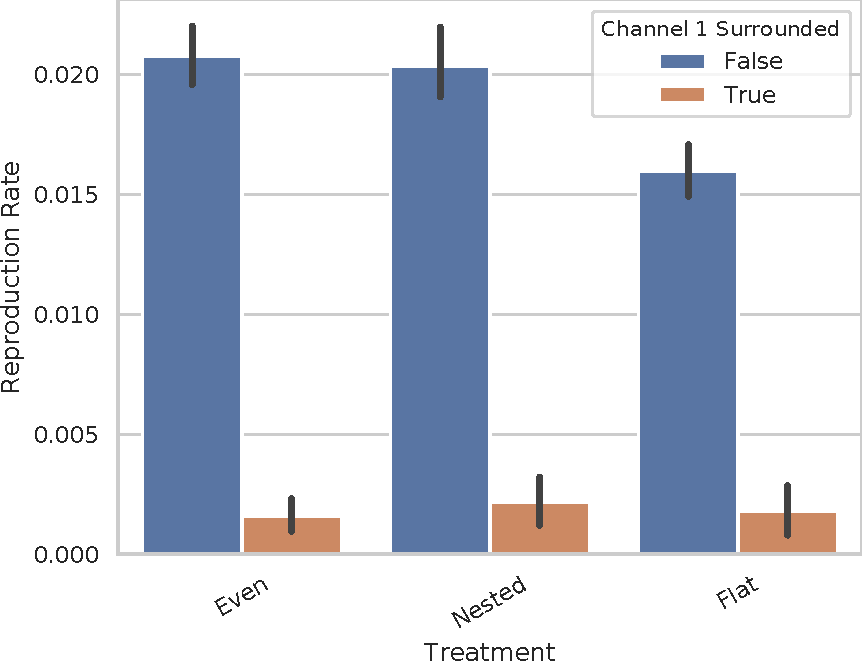
\includegraphics[width=\columnwidth]{reproduction/title=reproductive_labor_surrounded+_data_hathash_hash=4e1be4c5abfa4b05+_script_fullcat_hash=62ec0af515e8429d+_source_hash=ffbe01c-clean+ext=}

\caption{
TODO
}
\label{fig:reproduction_surrounted}
\end{center}
\end{figure}


Figure \ref{fig:reproduction_surrounded} shows cellular reproduction rates based on context in highest-level same-channel signaling networks.
In the nested and even treatments, this corresponded to the level-one channel and, in the flat treatment where no level-one channel was defined, this corresponded to the level-zero channel.
For all treatments, phenotypes with depressed interior cellular reproduction rates dominated across replicates ($p < 0.05$; $n=40$; bootstrap test).
[TODO just lookin' at non-overlapping 95\% CI's y'all]
All three treatments appear to be sufficient to select for reproductive cooperation among cells.

\subsection{Resource Sharing} \label{sec:resource-sharing}

\begin{figure*}[!htbp]
\begin{center}

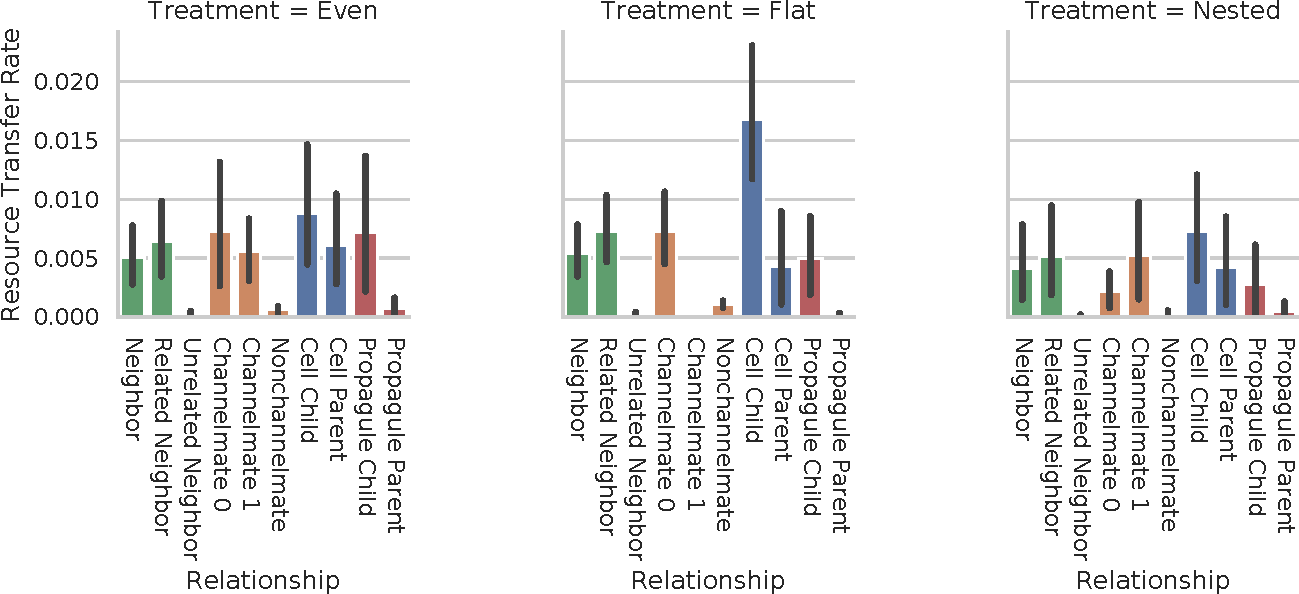
\includegraphics[width=\textwidth]{sharing/title=Resource_Transfer_Rate+_data_hathash_hash=e07865a0aee42cf7+_script_fullcat_hash=3612aad527ec4368+_source_hash=ffbe01c-clean+ext=}

\caption{
TODO
}
\label{fig:sharing}
\end{center}
\end{figure*}

\begin{figure*}[!htbp]
\begin{center}

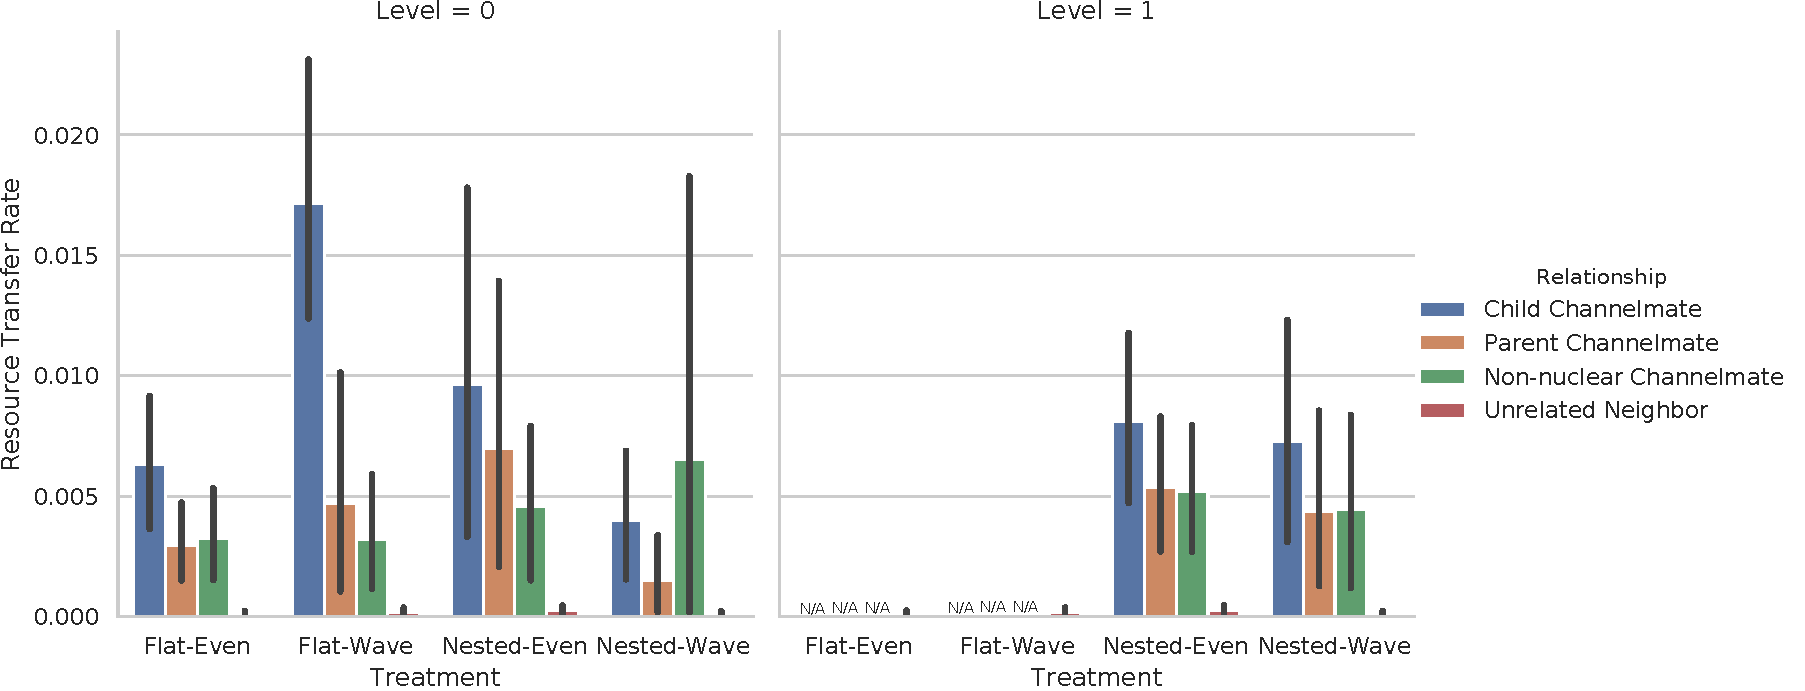
\includegraphics[width=\textwidth]{sharing/title=Resource_Transfer_Rate+_data_hathash_hash=2137e250b9d2b681+_script_fullcat_hash=86edbf4a4e5f34ed+_source_hash=53a2252-clean+ext=}

\caption{
Resource sharing to mutually exclusive sub-categories same-channel cellular neighbors: cellular child, cellular parent, and neither (``non-nuclear'').
Resource sharing to entirely non-related cells (no cell, channel, or propagule relation) is included for comparison.
Note that level-one groups are not defined in either of the flat treatments.
Error bars indicate 95\% confidence.
}
\label{fig:sharing_channelmate}
\end{center}
\end{figure*}


Figure \ref{fig:sharing} overviews evolved resource sharing behavior across cellular contexts.

Replicates in the flat treatment exhibit an especially elevated rate of resource sharing to cell children.
This could perhaps be due to an especial selective pressure to convey resource towards the group periphery.

Also, in the even and flat treatments, more resource was shared to neighbors within a cell's same-channel signaling network's propagule than to an unrelated neighbor ($p < 0.05$; $n=40$; bootstrap test).
Functional cooperation to directly further group reproduction therefore appears to have evolved commonly under these treatments.

Surprisingly, in the nested treatment resource was shared at a higher mean rate among high-level same-channel signaling groups than low-level groups.
This observation is likely due to replicates where level-one same-channel signaling groups were composed of single-cell level-zero same-channel signaling groups (where no or very few opportunities for level-zero resource sharing occurred).

Finally, under all treatments resource was transferred to channelmates at a significantly higher mean rate than to unrelated neighbors ($p < 0.05$; $n=40$; bootstrap test).
[TODO just lookin' at non-overlapping 95\% CI's y'all]
This observation suggests that functional cooperation within same-channel groups might have been a common evolutionary outcome under all three treatments.
However, it could potentially be an artifact of resource sharing between direct cellular kin.

Figure \ref{fig:sharing_channelmate} breaks same-channel resource-sharing apart by cellular kin relation.
In all three treatments, mean sharing to direct-kin channelmates was indeed greater than to other channelmates.
This cold be due to an evolutionary incentive to favor direct cell kin over other channelmates, group-level selection for asymmetric resource flow achieved by preferential sharing, or some combination of the two.
However, in all three treatments mean sharing to non-direct-kin channelmates was also significantly greater than resource sharing to unrelated neighbors ($p < 0.05$; $n=40$; bootstrap test).
[TODO just lookin' at non-overlapping 95\% CI's y'all]
Thus, all three treatments appear to be sufficient to select for functional cooperation among cells.

\subsection{Case Studies: Life Histories} \label{sec:life-histories}

Although functional and reproductive cooperation was ubiquitous among same-channel signaling networks, across replicates these outcomes were realized via diverse set of qualitiative life histories.
\begin{figure*}[!htbp]
\begin{center}

\begin{subfigure}[b]{\textwidth}
\centering
\begin{minipage}[t]{0.18\textwidth}
\centering
\adjincludegraphics[width=\textwidth, trim={{.66\width} {.66\width} {.0\width} {.0\width}}, clip]{lifecycle/transfer-paint/seed=1004+title=directional_propagule_viz+treat=resource-wave__channelsense-yes__nlev-two+update=1048896+_data_hathash_hash=06a65518d5588ef3+_script_fullcat_hash=8b1f57a580a67198+_source_hash=ffbe01c-clean+ext=}
Update 0
\end{minipage}
\begin{minipage}[t]{0.18\textwidth}
\centering
\adjincludegraphics[width=\textwidth, trim={{.66\width} {.66\width} {.0\width} {.0\width}}, clip]{lifecycle/transfer-paint/seed=1004+title=directional_propagule_viz+treat=resource-wave__channelsense-yes__nlev-two+update=1048928+_data_hathash_hash=06a65518d5588ef3+_script_fullcat_hash=8b1f57a580a67198+_source_hash=ffbe01c-clean+ext=}
Update 32
\end{minipage}
\begin{minipage}[t]{0.18\textwidth}
\centering
\adjincludegraphics[width=\textwidth, trim={{.66\width} {.66\width} {.0\width} {.0\width}}, clip]{lifecycle/transfer-paint/seed=1004+title=directional_propagule_viz+treat=resource-wave__channelsense-yes__nlev-two+update=1048960+_data_hathash_hash=06a65518d5588ef3+_script_fullcat_hash=8b1f57a580a67198+_source_hash=ffbe01c-clean+ext=}
Update 64
\end{minipage}
\begin{minipage}[t]{0.18\textwidth}
\centering
\adjincludegraphics[width=\textwidth, trim={{.66\width} {.66\width} {.0\width} {.0\width}}, clip]{lifecycle/transfer-paint/seed=1004+title=directional_propagule_viz+treat=resource-wave__channelsense-yes__nlev-two+update=1049024+_data_hathash_hash=06a65518d5588ef3+_script_fullcat_hash=8b1f57a580a67198+_source_hash=ffbe01c-clean+ext=}
Update 128
\end{minipage}
\begin{minipage}[t]{0.18\textwidth}
\centering
\adjincludegraphics[width=\textwidth, trim={{.66\width} {.66\width} {.0\width} {.0\width}}, clip]{lifecycle/transfer-paint/seed=1004+title=directional_propagule_viz+treat=resource-wave__channelsense-yes__nlev-two+update=1049408+_data_hathash_hash=06a65518d5588ef3+_script_fullcat_hash=8b1f57a580a67198+_source_hash=ffbe01c-clean+ext=}
Update 512
\end{minipage}
\caption{Spawn TODO}
\label{fig:TODO}
\end{subfigure}

\vspace{3ex}

\begin{subfigure}[b]{\textwidth}
\centering
\begin{minipage}[t]{0.18\textwidth}
\centering
\adjincludegraphics[width=\textwidth, trim={{.0\width} {.0\width} {.66\width} {.66\width}}, clip]{lifecycle/replace-paint/seed=1023+title=directional_propagule_viz+treat=resource-wave__channelsense-yes__nlev-two+update=1048576+_data_hathash_hash=39aa6b64134daefa+_script_fullcat_hash=8b1f57a580a67198+_source_hash=ffbe01c-clean+ext=}
Update 0
\end{minipage}
\begin{minipage}[t]{0.18\textwidth}
\centering
\adjincludegraphics[width=\textwidth, trim={{.0\width} {.0\width} {.66\width} {.66\width}}, clip]{lifecycle/replace-paint/seed=1023+title=directional_propagule_viz+treat=resource-wave__channelsense-yes__nlev-two+update=1048648+_data_hathash_hash=39aa6b64134daefa+_script_fullcat_hash=8b1f57a580a67198+_source_hash=ffbe01c-clean+ext=}
Update 72
\end{minipage}
\begin{minipage}[t]{0.18\textwidth}
\centering
\adjincludegraphics[width=\textwidth, trim={{.0\width} {.0\width} {.66\width} {.66\width}}, clip]{lifecycle/replace-paint/seed=1023+title=directional_propagule_viz+treat=resource-wave__channelsense-yes__nlev-two+update=1048720+_data_hathash_hash=39aa6b64134daefa+_script_fullcat_hash=8b1f57a580a67198+_source_hash=ffbe01c-clean+ext=}
Update 144
\end{minipage}
\begin{minipage}[t]{0.18\textwidth}
\centering
\adjincludegraphics[width=\textwidth, trim={{.0\width} {.0\width} {.66\width} {.66\width}}, clip]{lifecycle/replace-paint/seed=1023+title=directional_propagule_viz+treat=resource-wave__channelsense-yes__nlev-two+update=1048792+_data_hathash_hash=39aa6b64134daefa+_script_fullcat_hash=8b1f57a580a67198+_source_hash=ffbe01c-clean+ext=}
Update 216
\end{minipage}
\begin{minipage}[t]{0.18\textwidth}
\centering
\adjincludegraphics[width=\textwidth, trim={{.0\width} {.0\width} {.66\width} {.66\width}}, clip]{lifecycle/replace-paint/seed=1023+title=directional_propagule_viz+treat=resource-wave__channelsense-yes__nlev-two+update=1048864+_data_hathash_hash=39aa6b64134daefa+_script_fullcat_hash=8b1f57a580a67198+_source_hash=ffbe01c-clean+ext=}
Update 288
\end{minipage}
\caption{Replace TODO}
\label{fig:TODO}
\end{subfigure}

\vspace{3ex}

\begin{subfigure}[b]{\textwidth}
\centering
\begin{minipage}[t]{0.18\textwidth}
\centering
\adjincludegraphics[width=\textwidth, trim={{.0\width} {.66\width} {.66\width} {.0\width}}, clip]{lifecycle/burst-paint/seed=1034+title=directional_propagule_viz+treat=resource-wave__channelsense-yes__nlev-two+update=1048648+_data_hathash_hash=02a94757e9b17a36+_script_fullcat_hash=8b1f57a580a67198+_source_hash=ffbe01c-clean+ext=}
Update 0
\end{minipage}
\begin{minipage}[t]{0.18\textwidth}
\centering
\adjincludegraphics[width=\textwidth, trim={{.0\width} {.66\width} {.66\width} {.0\width}}, clip]{lifecycle/burst-paint/seed=1034+title=directional_propagule_viz+treat=resource-wave__channelsense-yes__nlev-two+update=1048744+_data_hathash_hash=02a94757e9b17a36+_script_fullcat_hash=8b1f57a580a67198+_source_hash=ffbe01c-clean+ext=}
Update 96
\end{minipage}
\begin{minipage}[t]{0.18\textwidth}
\centering
\adjincludegraphics[width=\textwidth, trim={{.0\width} {.66\width} {.66\width} {.0\width}}, clip]{lifecycle/burst-paint/seed=1034+title=directional_propagule_viz+treat=resource-wave__channelsense-yes__nlev-two+update=1048840+_data_hathash_hash=02a94757e9b17a36+_script_fullcat_hash=8b1f57a580a67198+_source_hash=ffbe01c-clean+ext=}
Update 192
\end{minipage}
\begin{minipage}[t]{0.18\textwidth}
\centering
\adjincludegraphics[width=\textwidth, trim={{.0\width} {.66\width} {.66\width} {.0\width}}, clip]{lifecycle/burst-paint/seed=1034+title=directional_propagule_viz+treat=resource-wave__channelsense-yes__nlev-two+update=1048936+_data_hathash_hash=02a94757e9b17a36+_script_fullcat_hash=8b1f57a580a67198+_source_hash=ffbe01c-clean+ext=}
Update 288
\end{minipage}
\begin{minipage}[t]{0.18\textwidth}
\centering
\adjincludegraphics[width=\textwidth, trim={{.0\width} {.66\width} {.66\width} {.0\width}}, clip]{lifecycle/burst-paint/seed=1034+title=directional_propagule_viz+treat=resource-wave__channelsense-yes__nlev-two+update=1049032+_data_hathash_hash=02a94757e9b17a36+_script_fullcat_hash=8b1f57a580a67198+_source_hash=ffbe01c-clean+ext=}
Update 384
\end{minipage}
\caption{Burst TODO}
\label{fig:TODO}
\end{subfigure}

\vspace{3ex}

\begin{subfigure}[b]{\textwidth}
\centering
\begin{minipage}[t]{0.18\textwidth}
\centering
\adjincludegraphics[width=\textwidth, trim={{.5\width} {.33\width} {.17\width} {.33\width}}, clip]{lifecycle/cell-paint/seed=1026+title=directional_daughter_viz+treat=resource-wave__channelsense-yes__nlev-two+update=1048576+_data_hathash_hash=a22f7463ee6886d7+_script_fullcat_hash=ef865c98cd111636+_source_hash=ffbe01c-clean+ext=}
Update 0
\end{minipage}
\begin{minipage}[t]{0.18\textwidth}
\centering
\adjincludegraphics[width=\textwidth, trim={{.5\width} {.33\width} {.17\width} {.33\width}}, clip]{lifecycle/cell-paint/seed=1026+title=directional_daughter_viz+treat=resource-wave__channelsense-yes__nlev-two+update=1048704+_data_hathash_hash=a22f7463ee6886d7+_script_fullcat_hash=ef865c98cd111636+_source_hash=ffbe01c-clean+ext=}
Update 128
\end{minipage}
\begin{minipage}[t]{0.18\textwidth}
\centering
\adjincludegraphics[width=\textwidth, trim={{.5\width} {.33\width} {.17\width} {.33\width}}, clip]{lifecycle/cell-paint/seed=1026+title=directional_daughter_viz+treat=resource-wave__channelsense-yes__nlev-two+update=1048832+_data_hathash_hash=a22f7463ee6886d7+_script_fullcat_hash=ef865c98cd111636+_source_hash=ffbe01c-clean+ext=}
Update 256
\end{minipage}
\begin{minipage}[t]{0.18\textwidth}
\centering
\adjincludegraphics[width=\textwidth, trim={{.5\width} {.33\width} {.17\width} {.33\width}}, clip]{lifecycle/cell-paint/seed=1026+title=directional_daughter_viz+treat=resource-wave__channelsense-yes__nlev-two+update=1048960+_data_hathash_hash=a22f7463ee6886d7+_script_fullcat_hash=ef865c98cd111636+_source_hash=ffbe01c-clean+ext=}
Update 384
\end{minipage}
\begin{minipage}[t]{0.18\textwidth}
\centering
\adjincludegraphics[width=\textwidth, trim={{.5\width} {.33\width} {.17\width} {.33\width}}, clip]{lifecycle/cell-paint/seed=1026+title=directional_daughter_viz+treat=resource-wave__channelsense-yes__nlev-two+update=1049088+_data_hathash_hash=a22f7463ee6886d7+_script_fullcat_hash=ef865c98cd111636+_source_hash=ffbe01c-clean+ext=}
Update 512
\end{minipage}
\caption{Cellular TODO}
\label{fig:TODO}
\end{subfigure}


\caption{
TODO
same-channel signaling networks
}
\label{fig:ko-apoptosis}
\end{center}
\end{figure*}


Figure \ref{fig:lifecycle} compares four life histories evolved under the nested treatment.
In example \ref{fig:lifecycle-coalesce}, propagules repeatedly bud off of parent groups to yield a larger network of persistent parent-child cooperators.
In example, \ref{fig:lifecycle-sweep}, propagules are generated at the extremities of parent groups and then rapidly replace most or all of the parent group.
In example, \ref{fig:lifecycle-burst}, propagules are generated at the interior of a parent group and replace it from the inside out.
Finally, example \ref{fig:lifecycle-naive} profiles a more naive life history in which --- beyond the cellular progenitor of a propagule group --- the parent and propagule groups exhibit no special cooperative relationship.

\subsection{Case Study: Gene Regulation} \label{sec:gene-regulation}

\begin{figure}[!htbp]
\begin{center}

\begin{subfigure}[b]{\linewidth}
\begin{center}

\begin{minipage}[t]{0.18\linewidth}
\centering
\vspace{0pt} % for alignment
\adjincludegraphics[width=\textwidth, trim={{.0\width} {.77\width} {.79\width} {.02\width}}, clip]{lifecycle/burst-paint/seed=1034+title=directional_channel_grayscale_viz+treat=resource-wave__channelsense-yes__nlev-two+update=1048648+_data_hathash_hash=ca8ad21d3b30b939+_script_fullcat_hash=602c0d0c070e9202+_source_hash=53a2252-clean+ext=}
\footnotesize Update 0
\end{minipage}
\begin{minipage}[t]{0.18\linewidth}
\centering
\vspace{0pt} % for alignment
\adjincludegraphics[width=\textwidth, trim={{.0\width} {.77\width} {.79\width} {.02\width}}, clip]{lifecycle/burst-paint/seed=1034+title=directional_channel_grayscale_viz+treat=resource-wave__channelsense-yes__nlev-two+update=1048744+_data_hathash_hash=ca8ad21d3b30b939+_script_fullcat_hash=602c0d0c070e9202+_source_hash=53a2252-clean+ext=}
\footnotesize 96
\end{minipage}
\begin{minipage}[t]{0.18\linewidth}
\centering
\vspace{0pt} % for alignment
\adjincludegraphics[width=\textwidth, trim={{.0\width} {.77\width} {.79\width} {.02\width}}, clip]{lifecycle/burst-paint/seed=1034+title=directional_channel_grayscale_viz+treat=resource-wave__channelsense-yes__nlev-two+update=1048840+_data_hathash_hash=ca8ad21d3b30b939+_script_fullcat_hash=602c0d0c070e9202+_source_hash=53a2252-clean+ext=}
\footnotesize 192
\end{minipage}
\begin{minipage}[t]{0.18\linewidth}
\centering
\vspace{0pt} % for alignment
\adjincludegraphics[width=\textwidth, trim={{.0\width} {.77\width} {.79\width} {.02\width}}, clip]{lifecycle/burst-paint/seed=1034+title=directional_channel_grayscale_viz+treat=resource-wave__channelsense-yes__nlev-two+update=1048936+_data_hathash_hash=ca8ad21d3b30b939+_script_fullcat_hash=602c0d0c070e9202+_source_hash=53a2252-clean+ext=}
\footnotesize 288
\end{minipage}
\begin{minipage}[t]{0.18\linewidth}
\centering
\vspace{0pt} % for alignment
\adjincludegraphics[width=\textwidth, trim={{.0\width} {.77\width} {.79\width} {.02\width}}, clip]{lifecycle/burst-paint/seed=1034+title=directional_channel_grayscale_viz+treat=resource-wave__channelsense-yes__nlev-two+update=1049032+_data_hathash_hash=ca8ad21d3b30b939+_script_fullcat_hash=602c0d0c070e9202+_source_hash=53a2252-clean+ext=}
\footnotesize 384
\end{minipage}
\caption{Wild type timelapse}
\label{fig:wt_timelapse}
\end{center}
\end{subfigure}

\vspace{2ex}

\begin{subfigure}[b]{\linewidth}
\begin{center}

\begin{minipage}[t]{0.30\linewidth}
\centering
\vspace{0pt} % for alignment
% adapted from https://tex.stackexchange.com/a/186476
\begin{tikzpicture}
\node[anchor=south west,inner sep=0] (image) at (0,0) { \adjincludegraphics[width=\linewidth, trim={{.25\width} {.20\width} {.5\width} {.55\width}}, clip]{knockout/interior_propagule/wildtype/seed=1+title=directional_regulator_viz+treat=resource-wave__channelsense-yes__nlev-two+update=8188+_data_hathash_hash=8b493febd79aad1f+_script_fullcat_hash=90718bb0c6ec4dbd+_source_hash=53a2252-clean+ext=}
};
\begin{scope}[x={(image.south east)},y={(image.north west)}]
  \draw [-stealth, yellow] (0.35,0.59) -- ++(0.05,-0.05);
  \draw [-stealth, yellow] (0.01,0.39) -- ++(0.05,-0.05);
  \draw [-stealth, yellow] (0.68,0.39) -- ++(0.05,-0.05);
  \draw [-stealth, yellow] (0.62,0.32) -- ++(0.05,-0.05);
\end{scope}
\end{tikzpicture}
\footnotesize Wild type
\end{minipage}
\begin{minipage}[t]{0.30\linewidth}
\centering
\vspace{0pt} % for alignment
\adjincludegraphics[width=\linewidth, trim={{.5\width} {.5\width} {.25\width} {.25\width}}, clip]{knockout/interior_propagule/propaguleknockout/seed=1+title=directional_regulator_viz+treat=resource-wave__channelsense-yes__nlev-two+update=8188+_data_hathash_hash=2b6711db47fb5887+_script_fullcat_hash=90718bb0c6ec4dbd+_source_hash=53a2252-clean+ext=}
\footnotesize Propagule knockout
\end{minipage}
\begin{minipage}[t]{0.30\linewidth}
\centering
\vspace{0pt} % for alignment
\adjincludegraphics[width=\linewidth, trim={{.5\width} {.5\width} {.25\width} {.25\width}}, clip]{knockout/interior_propagule/regulationknockout/seed=1+title=directional_regulator_viz+treat=resource-wave__channelsense-yes__nlev-two+update=8188+_data_hathash_hash=11ab5cdd47ed18c7+_script_fullcat_hash=90718bb0c6ec4dbd+_source_hash=53a2252-clean+ext=}
\footnotesize Regulation knockout
\end{minipage}

\caption{Regulation visualizations}
\label{fig:regulation_visualizations}

\end{center}
\end{subfigure}

\begin{minipage}[t]{\linewidth}
\centering
\vspace{0pt} % for alignment
\begin{subfigure}[b]{\linewidth}
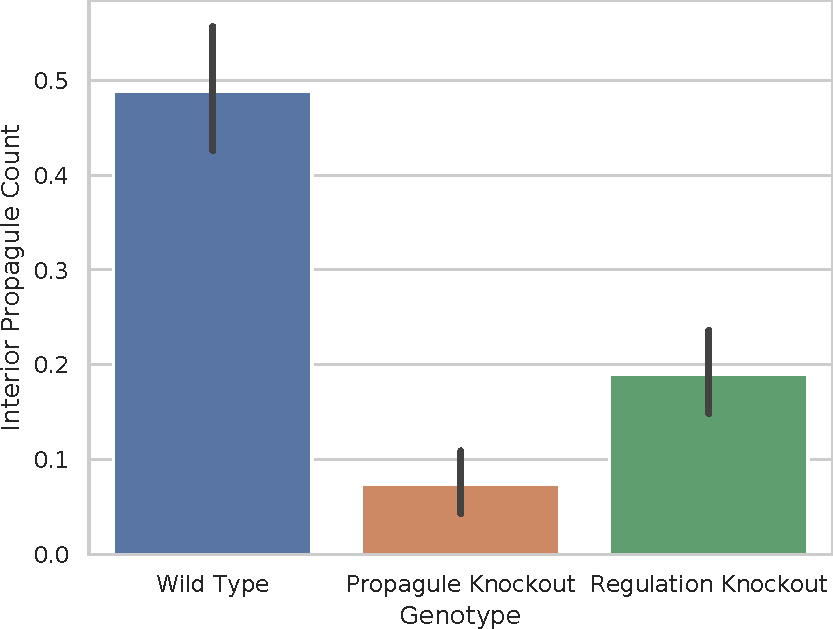
\includegraphics[width=\linewidth]{knockout/interior_propagule/title=interior_propagules+_data_hathash_hash=bb0fa6254f1b7398+_script_fullcat_hash=f738b363bea8c98a+_source_hash=53a2252-clean+ext=}%
\caption{Interior propagule rate by genotype}
\label{fig:interior_propagule_rate}
\end{subfigure}
\end{minipage}%
\hspace*{\fill}


\caption{
Analysis of a wild type strain evolved under the ``Nested-Wave'' treatment exhibiting interior propagule generation, comparing against knockouts of gene regulation and explicitly propagule-generating reproduction instructions.
Figure \ref{fig:wt_timelapse} traces the wild type life history.
Level-one groups are by differentiated by grayscale tone and separated by solid black borders.
Level-zero groups are by separated by dashed gray borders.
In each example, the focal parent level-one group is colored purple and the focal offspring group orange.
Figure \ref{fig:regulation_visualizations} depicts gene regulation at each of a cell's four directional SignalGP instances using a PCA mapping from regulatory state to three-dimensional RGB coordinates, calculated uniquely for each level-one same-channel signaling group.
Black borders divide level-one same-channel signaling groups and white borders divide level-zero same-channel signaling groups.
Endogenous daughter groups annotated with yellow arrows.
Figure \ref{fig:interior_propagule_rate} compares the mean number of interior propagules observed per level-one same-channel signaling group.
Error bars indicate 95\% confidence.
View an animation of wild type gene regulation at \url{https://mmore500.com/hopto/t}.
View the wild type strain in a live in-browser simulation at \url{https://mmore500.com/hopto/g}.
}
\label{fig:ko-interior_propagule}
\end{center}
\end{figure}


What mechanism determines the localization and timing of the propagule placement obseved in life history example \ref{fig:lifecycle-burst}?
This wild type strain exhibits an irregular, but somewhat concentric, spatial pattern of gene regulation illustrated in Figure \ref{fig:interior_propagule-wt}.
In time-series animation, provided in supplementary material, gene regulation appears to fluctuate dynamically.

To assess mechanistic and adaptive role of gene regulation in this strain, we prepared two knockout strains.
In the first, all gene regulation instructions were replaced with \textbf{Nop} instructions (so that gene regulation values would remain default).
In the second, the reproduction instructions to spawn a propagule were replaced with \textbf{Nop} instructions.
Figures \ref{fig:interior_propagule-ko-regulation} and \ref{fig:interior_propagule-ko-propagule} depict the gene regulation phenotypes of these strains.

Figure \ref{fig:interior_propagule_rate} compares interior propagule generation between the strains, confirming the direct mechanistic role of gene regulation in promoting interior propagule generation ($p < 0.05$; bootstrap test).
[TODO just lookin' at non-overlapping 95\% CI's y'all]

In head-to-head match-ups, the wild type strain outcompetes both the regulation-knockout ($20/20$; $p < 0.001$; two-tailed exact test) and the propagule-knockout strains
($20/20$; $p < 0.001$; two-tailed exact test).
The deficiency of the propagule-knockout strain confirms the adaptive role of interior propagule generation.
Likewise, the deficiency of the regulation-knockout strain affirms the adaptive role of gene regulation in the focal wild type strain.

\subsection{Case Study: Gradient-conditioned Cell Behavior} \label{sec:gradient-conditioned-behavior}

\begin{figure}[!htbp]
\begin{center}

\centering

\hspace*{\fill}%
\begin{minipage}[t]{0.05\columnwidth}
\vspace{0pt} % for alignment
\rotatebox{90}{Resource Stockpile}%
\end{minipage}%
\hfill
\begin{minipage}[t]{0.45\columnwidth}
\centering
\vspace{0pt} % for alignment
\adjincludegraphics[width=\textwidth, trim={{.0\width} {.0\width} {.5\width} {.5\width}}, clip]{knockout/stockpiletrigger-sharing/wildtype/seed=1+title=stockpile_viz+treat=resource-wave__channelsense-yes__nlev-two+update=7172+_data_hathash_hash=d856da4ae5863122+_script_fullcat_hash=4c8152cbf92e0da6+_source_hash=53a2252-clean+ext=}%
\end{minipage}%
\hfill
\begin{minipage}[t]{0.45\columnwidth}
\centering
\vspace{0pt} % for alignment
\adjincludegraphics[width=\textwidth, trim={{.0\width} {.0\width} {.5\width} {.5\width}}, clip]{knockout/stockpiletrigger-sharing/knockout/seed=1+title=stockpile_viz+treat=resource-wave__channelsense-yes__nlev-two+update=7172+_data_hathash_hash=6ab6ade50c5344bc+_script_fullcat_hash=4c8152cbf92e0da6+_source_hash=53a2252-clean+ext=}%
\end{minipage}%
\hspace*{\fill}


\hspace*{\fill}%
\begin{minipage}[t]{0.05\columnwidth}
\vspace{0pt} % for alignment
\rotatebox{90}{Resource Sharing}%
\end{minipage}%
\hfill
\begin{minipage}[t]{0.45\columnwidth}
\centering
\vspace{0pt} % for alignment
\adjincludegraphics[width=\textwidth, trim={{.0\width} {.0\width} {.5\width} {.5\width}}, clip]{knockout/stockpiletrigger-sharing/wildtype/seed=1+title=directional_sharing_viz+treat=resource-wave__channelsense-yes__nlev-two+update=7172+_data_hathash_hash=d856da4ae5863122+_script_fullcat_hash=3a1e851383e0ffd4+_source_hash=53a2252-clean+ext=}%
\end{minipage}%
\hfill
\begin{minipage}[t]{0.45\columnwidth}
\centering
\vspace{0pt} % for alignment
\adjincludegraphics[width=\textwidth, trim={{.0\width} {.0\width} {.5\width} {.5\width}}, clip]{knockout/stockpiletrigger-sharing/knockout/seed=1+title=directional_sharing_viz+treat=resource-wave__channelsense-yes__nlev-two+update=7172+_data_hathash_hash=6ab6ade50c5344bc+_script_fullcat_hash=3a1e851383e0ffd4+_source_hash=53a2252-clean+ext=}%
\end{minipage}%
\hspace*{\fill}

\vspace{1.0ex}

\hspace*{\fill}%
\begin{minipage}[t]{0.05\columnwidth}
\vspace{0pt} % for alignment
\end{minipage}%
\hfill
\begin{minipage}[t]{0.45\columnwidth}
\centering
\vspace{0pt} % for alignment
Wild Type
\end{minipage}%
\hfill
\begin{minipage}[t]{0.45\columnwidth}
\centering
\vspace{0pt} % for alignment
Messaging Knockout
\end{minipage}%
\hspace*{\fill}

\vspace{1.0ex}

\caption{
Visualization of phenotypic traits of a wild type strain evolved under the ``Nested-Wave''' treatment and corresponding resource-sensing knockout strain.
In the resource-sharing visualization, color coding represents the amount of incoming shared resource.
White represents no incoming messages and the magenta to blue gradient runs from one incoming message to the maximum observed incoming message traffic.
In the resource stockpile visualization, white represents zero-resource stockpiles, blue represents stockpiles with just under enough resource to reproduce, green represents stockpiles with enough resource to reproduce, and yellow represents more than enough resource to reproduce.
Black borders divide level-one same-channel signaling groups and white borders divide level-zero same-channel signaling groups.
}
\label{fig:ko-stockpiletrigger-sharing}
\end{center}
\end{figure}


We discovered a strain using resource concentration to regulate directionality of resource sharing in a manner somewhat akin to morphogenic patterning.
This strain's wild type outcompeted a variant with knock out of capacity to asses relative richness of neighboring resource stockpiles ($20/20$; $p < 0.001$; two-tailed exact test).
Figure \ref{fig:ko-stockpiletrigger-sharing} contrasts the wild type resource-sharing phenotype  with the more sparse knockout resource-sharing phenotype.

\subsection{Case Study: Morphology} \label{sec:morphology}

\begin{figure}[!htbp]
\begin{center}

\hspace*{\fill}%
\begin{minipage}[t]{0.45\columnwidth}
\centering
\vspace{0pt} % for alignment
\begin{subfigure}[b]{\textwidth}
\adjincludegraphics[width=\textwidth, trim={{.0\width} {.0\width} {.5\width} {.5\width}}, clip]{knockout/morphology/wildtype/seed=1+title=channel_viz+treat=resource-even__channelsense-yes__nlev-two+update=8188+_data_hathash_hash=cb64cdf045bc6049+_script_fullcat_hash=7e789c981e3d0e4f+_source_hash=53a2252-clean+ext=}
\caption{Wild type}
\label{fig:morphology-wt}
\end{subfigure}
\end{minipage}%
\hfill
\begin{minipage}[t]{0.45\columnwidth}
\centering
\vspace{0pt} % for alignment
\begin{subfigure}[b]{\textwidth}
\adjincludegraphics[width=\textwidth, trim={{.0\width} {.0\width} {.5\width} {.5\width}}, clip]{knockout/morphology/knockout/seed=1+title=channel_viz+treat=resource-even__channelsense-yes__nlev-two+update=8188+_data_hathash_hash=9a4119947348e91d+_script_fullcat_hash=7e789c981e3d0e4f+_source_hash=53a2252-clean+ext=}%
\caption{Messaging knockout}
\label{fig:morphology-ko}
\end{subfigure}
\end{minipage}%
\hspace*{\fill}

\hspace*{\fill}%
\begin{minipage}[t]{\columnwidth}
\centering
\vspace{0pt} % for alignment
\begin{subfigure}[b]{\textwidth}
\adjincludegraphics[width=\textwidth]{knockout/morphology/title=group_shape+_data_hathash_hash=cb1733796dea778f+_script_fullcat_hash=68cf35a1759c64ac+_source_hash=53a2252-clean+ext=}
\caption{Distribution of level-zero same-channel neighbor counts}
\label{fig:morphology-shape}
\end{subfigure}
\end{minipage}%
\hspace*{\fill}

\caption{
Comparison of a wild type strain with stringy level-zero same-channel signaling networks and the corresponding intracellular-messaging knockout strain.
Subfigures \ref{fig:morphology-wt} and \ref{fig:morphology-ko} visualize same-channel signaling network layouts;
color hue denotes and black borders divide level-one same-channel signaling networks while
color saturation denotes and white borders divide level-zero same-channel signaling networks.
Subfigure \ref{fig:morphology-shape} quantifies the morphological effect of the
intracellular-messaging knockout.
Error bars indicate 95\% confidence.
}
\label{fig:ko-morphology}
\end{center}
\end{figure}


One of the more striking examples of genetically-encoded same-channel signaling network patterning, in which level-zero same-channel signaling groups arranged as elongated strings, arose in a even treatment replicate.
Figure \ref{fig:morphology-wt} provides a snapshot of this strain's same-channel signaling morphology.
Knocking out intracell messaging disrupts the stringy arrangement of same-channel signaling groups, shown in Figure \ref{fig:morphology-ko}.
Figure \ref{fig:morphology-shape} confirms the genetic basis of the trait.
Cells from the wild-type strain more often neighbor only zero or one level-zero same-channel cells ($p < 0.05$; bootstrap test).
[TODO just lookin' at non-overlapping 95\% CI's y'all]
In contrast, knockout strain cells more frequently neighbor three or four level-zero same-channel cells ($p < 0.05$; bootstrap test).
[TODO just lookin' at non-overlapping 95\% CI's y'all]

However, competition experiments between the wild type and knockout strain failed to establish a fitness differential ($6/20$).
Thus, it seems this trait emerged either by drift, as the genetic background of a selective sweep, or --- perhaps less likely --- was advantageous against a divergent competitor earlier in evolutionary history.

\subsection{Case Studies: Cell-cell Messaging} \label{sec:cell-cell-messaging}

\begin{figure*}[!htbp]
\begin{center}

\begin{minipage}[t]{\columnwidth}
\hspace*{\fill}%
\begin{minipage}[t]{0.05\columnwidth}
\vspace{0pt} % for alignment
\rotatebox{90}{Messaging}%
\end{minipage}%
\hfill
\begin{minipage}[t]{0.45\columnwidth}
\centering
\vspace{0pt} % for alignment
\adjincludegraphics[width=\textwidth, trim={{.0\width} {.0\width} {.5\width} {.5\width}}, clip]{knockout/intermessaging-sharing/wildtype/seed=1+title=directional_messaging_viz+treat=resource-wave__channelsense-yes__nlev-onebig+update=7172+_data_hathash_hash=f9e2a8ff33bf7745+_script_fullcat_hash=6b7e0389992dd616+_source_hash=53a2252-clean+ext=}%
\end{minipage}%
\hfill
\begin{minipage}[t]{0.45\columnwidth}
\centering
\vspace{0pt} % for alignment
\adjincludegraphics[width=\textwidth, trim={{.0\width} {.0\width} {.5\width} {.5\width}}, clip]{knockout/intermessaging-sharing/knockout/seed=1+title=directional_messaging_viz+treat=resource-wave__channelsense-yes__nlev-onebig+update=7172+_data_hathash_hash=ffdeb1c77dd012e1+_script_fullcat_hash=6b7e0389992dd616+_source_hash=53a2252-clean+ext=}%
\end{minipage}%
\hspace*{\fill}

\hspace*{\fill}%
\begin{minipage}[t]{0.05\columnwidth}
\vspace{0pt} % for alignment
\rotatebox{90}{Resource Sharing}%
\end{minipage}%
\hfill
\begin{minipage}[t]{0.45\columnwidth}
\centering
\vspace{0pt} % for alignment
\adjincludegraphics[width=\textwidth, trim={{.0\width} {.0\width} {.5\width} {.5\width}}, clip]{knockout/intermessaging-sharing/wildtype/seed=1+title=directional_sharing_viz+treat=resource-wave__channelsense-yes__nlev-onebig+update=7172+_data_hathash_hash=f9e2a8ff33bf7745+_script_fullcat_hash=3a1e851383e0ffd4+_source_hash=53a2252-clean+ext=}%
\end{minipage}%
\hfill
\begin{minipage}[t]{0.45\columnwidth}
\centering
\vspace{0pt} % for alignment
\adjincludegraphics[width=\textwidth, trim={{.0\width} {.0\width} {.5\width} {.5\width}}, clip]{knockout/intermessaging-sharing/knockout/seed=1+title=directional_sharing_viz+treat=resource-wave__channelsense-yes__nlev-onebig+update=7172+_data_hathash_hash=ffdeb1c77dd012e1+_script_fullcat_hash=3a1e851383e0ffd4+_source_hash=53a2252-clean+ext=}%
\end{minipage}%
\hspace*{\fill}

\hspace*{\fill}%
\begin{minipage}[t]{0.05\columnwidth}
\vspace{0pt} % for alignment
\rotatebox{90}{Resource Stockpile}%
\end{minipage}%
\hfill
\begin{minipage}[t]{0.45\columnwidth}
\centering
\vspace{0pt} % for alignment
\adjincludegraphics[width=\textwidth, trim={{.0\width} {.0\width} {.5\width} {.5\width}}, clip]{knockout/intermessaging-sharing/wildtype/seed=1+title=stockpile_viz+treat=resource-wave__channelsense-yes__nlev-onebig+update=7172+_data_hathash_hash=f9e2a8ff33bf7745+_script_fullcat_hash=4c8152cbf92e0da6+_source_hash=53a2252-clean+ext=}%
\end{minipage}%
\hfill
\begin{minipage}[t]{0.45\columnwidth}
\centering
\vspace{0pt} % for alignment
\adjincludegraphics[width=\textwidth, trim={{.0\width} {.0\width} {.5\width} {.5\width}}, clip]{knockout/intermessaging-sharing/knockout/seed=1+title=stockpile_viz+treat=resource-wave__channelsense-yes__nlev-onebig+update=7172+_data_hathash_hash=ffdeb1c77dd012e1+_script_fullcat_hash=4c8152cbf92e0da6+_source_hash=53a2252-clean+ext=}%
\end{minipage}%
\hspace*{\fill}

\vspace{1.0ex}

\hspace*{\fill}%
\begin{minipage}[t]{0.05\columnwidth}
\vspace{0pt} % for alignment
\end{minipage}%
\hfill
\begin{minipage}[t]{0.45\columnwidth}
\centering
\vspace{0pt} % for alignment
Wild Type
\end{minipage}%
\hfill
\begin{minipage}[t]{0.45\columnwidth}
\centering
\vspace{0pt} % for alignment
Messaging Knockout
\end{minipage}%
\hspace*{\fill}

\vspace{1.0ex}

\begin{subfigure}{\columnwidth}
  \caption{Phenotype visualizations}
\end{subfigure}

\end{minipage}%
\begin{minipage}[t]{\columnwidth}

\hspace*{\fill}%
\begin{minipage}[t]{\textwidth}
\centering
\vspace{0pt} % for alignment
\begin{subfigure}[b]{\textwidth}
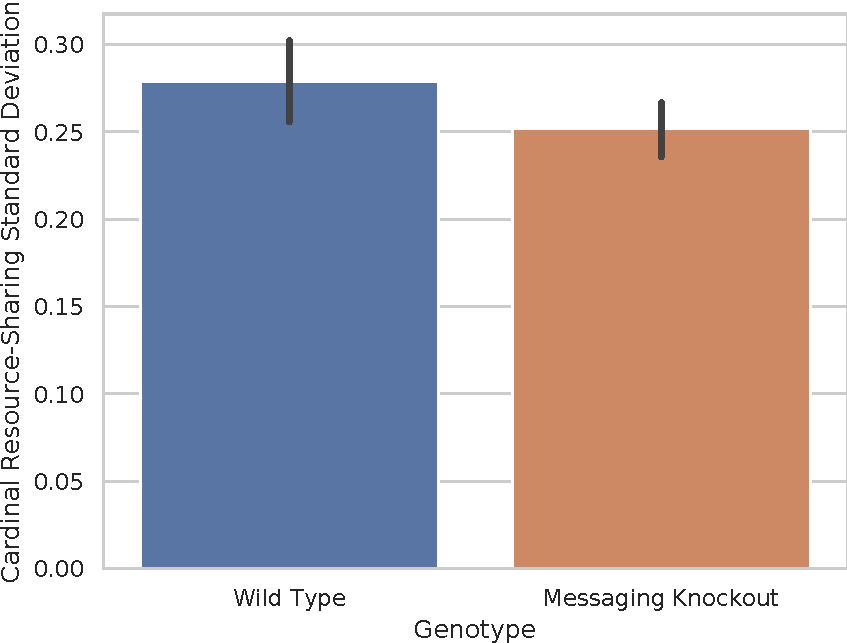
\includegraphics[width=\textwidth]{knockout/intermessaging-sharing/title=sharingdirection+_data_hathash_hash=59f6520a17fb3ad8+_script_fullcat_hash=97aad8dce5e50084+_source_hash=53a2252-clean+ext=}%
\caption{Net sharing direction variance}
\label{fig:TODO}
\end{subfigure}
\end{minipage}%
\hfill
\begin{minipage}[t]{\textwidth}
\centering
\vspace{0pt} % for alignment
\begin{subfigure}[b]{\textwidth}
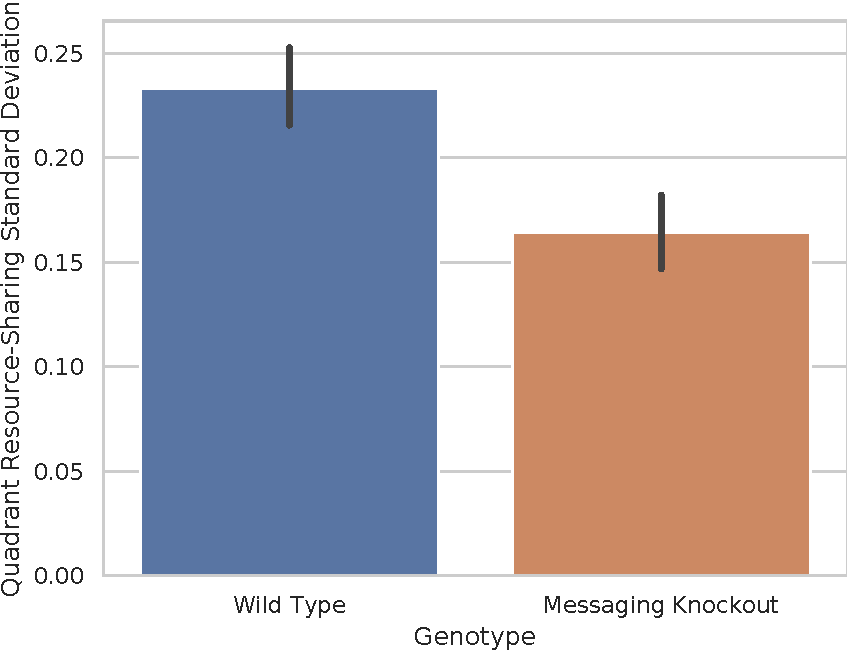
\includegraphics[width=\textwidth]{knockout/intermessaging-sharing/title=sharingquadrant+_data_hathash_hash=586f3c805332c323+_script_fullcat_hash=6e8aa37a96d9d7a9+_source_hash=53a2252-clean+ext=}%
\caption{Net sharing localization variance}
\label{fig:TODO}
\end{subfigure}
\end{minipage}%
\hfill
\begin{minipage}[t]{\textwidth}
\centering
\vspace{0pt} % for alignment
\begin{subfigure}[b]{\textwidth}
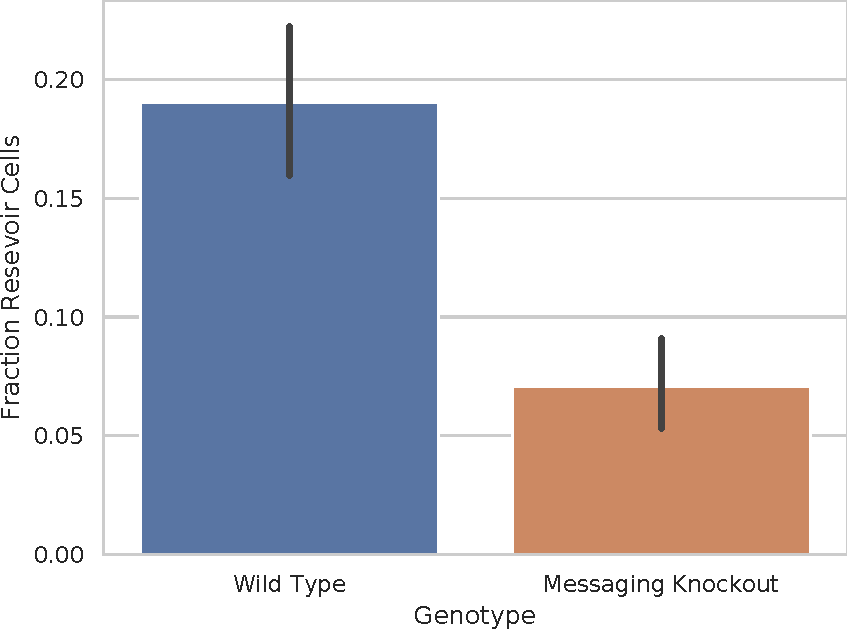
\includegraphics[width=\textwidth]{knockout/intermessaging-sharing/title=fractionresevoir+_data_hathash_hash=7ce9af7e8fe0699b+_script_fullcat_hash=da31ee3af7ae0208+_source_hash=53a2252-clean+ext=}%
\caption{Fraction of cells with enough resource to reproduce}
\label{fig:TODO}
\end{subfigure}
\end{minipage}%
\hspace*{\fill}
\end{minipage}

\caption{
TODO
}
\label{fig:ko-apoptosis}
\end{center}
\end{figure*}


\begin{figure*}[!htbp]
\begin{center}


\begin{minipage}[t]{\columnwidth}
\centering
\hspace*{\fill}%
\begin{minipage}[t]{0.05\columnwidth}
\vspace{0pt} % for alignment
\rotatebox{90}{Messaging}%
\end{minipage}%
\hfill
\begin{minipage}[t]{0.45\columnwidth}
\centering
\vspace{0pt} % for alignment
\adjincludegraphics[width=\textwidth, trim={{.66\width} {.66\width} {.0\width} {.0\width}}, clip]{knockout/intermessaging-intergroup_border/wildtype/seed=1+title=directional_messaging_viz+treat=resource-wave__channelsense-yes__nlev-two+update=7168+_data_hathash_hash=3895dfa0dd602b4c+_script_fullcat_hash=6b7e0389992dd616+_source_hash=53a2252-clean+ext=}%
\end{minipage}%
\hfill
\begin{minipage}[t]{0.45\columnwidth}
\centering
\vspace{0pt} % for alignment
\adjincludegraphics[width=\textwidth, trim={{.66\width} {.66\width} {.0\width} {.0\width}}, clip]{knockout/intermessaging-intergroup_border/knockout/seed=1+title=directional_messaging_viz+treat=resource-wave__channelsense-yes__nlev-two+update=7168+_data_hathash_hash=24546cc614406803+_script_fullcat_hash=6b7e0389992dd616+_source_hash=53a2252-clean+ext=}%
\end{minipage}%
\hspace*{\fill}

\hspace*{\fill}%
\begin{minipage}[t]{0.05\columnwidth}
\vspace{0pt} % for alignment
\rotatebox{90}{Parent-Propagule}%
\end{minipage}%
\hfill
\begin{minipage}[t]{0.45\columnwidth}
\centering
\vspace{0pt} % for alignment
\adjincludegraphics[width=\textwidth, trim={{.66\width} {.66\width} {.0\width} {.0\width}}, clip]{knockout/intermessaging-intergroup_border/wildtype/seed=1+title=directional_propagule_viz+treat=resource-wave__channelsense-yes__nlev-two+update=7168+_data_hathash_hash=3895dfa0dd602b4c+_script_fullcat_hash=8b1f57a580a67198+_source_hash=53a2252-clean+ext=}%
\end{minipage}%
\hfill
\begin{minipage}[t]{0.45\columnwidth}
\centering
\vspace{0pt} % for alignment
\adjincludegraphics[width=\textwidth, trim={{.66\width} {.66\width} {.0\width} {.0\width}}, clip]{knockout/intermessaging-intergroup_border/knockout/seed=1+title=directional_propagule_viz+treat=resource-wave__channelsense-yes__nlev-two+update=7168+_data_hathash_hash=24546cc614406803+_script_fullcat_hash=8b1f57a580a67198+_source_hash=53a2252-clean+ext=}%
\end{minipage}%
\hspace*{\fill}

\hspace*{\fill}%
\begin{minipage}[t]{0.05\columnwidth}
\vspace{0pt} % for alignment
\rotatebox{90}{Resource Sharing}%
\end{minipage}%
\hfill
\begin{minipage}[t]{0.45\columnwidth}
\centering
\vspace{0pt} % for alignment
\adjincludegraphics[width=\textwidth, trim={{.66\width} {.66\width} {.0\width} {.0\width}}, clip]{knockout/intermessaging-intergroup_border/wildtype/seed=1+title=directional_sharing_viz+treat=resource-wave__channelsense-yes__nlev-two+update=7172+_data_hathash_hash=3895dfa0dd602b4c+_script_fullcat_hash=3a1e851383e0ffd4+_source_hash=53a2252-clean+ext=}%
\end{minipage}%
\hfill
\begin{minipage}[t]{0.45\columnwidth}
\centering
\vspace{0pt} % for alignment
\adjincludegraphics[width=\textwidth, trim={{.66\width} {.66\width} {.0\width} {.0\width}}, clip]{knockout/intermessaging-intergroup_border/knockout/seed=1+title=directional_sharing_viz+treat=resource-wave__channelsense-yes__nlev-two+update=7172+_data_hathash_hash=24546cc614406803+_script_fullcat_hash=3a1e851383e0ffd4+_source_hash=53a2252-clean+ext=}%
\end{minipage}%
\hspace*{\fill}

% \hspace*{\fill}%
% \begin{minipage}[t]{0.05\columnwidth}
% \vspace{0pt} % for alignment
% \rotatebox{90}{Resource Stockpile}%
% \end{minipage}%
% \hfill
% \begin{minipage}[t]{0.45\columnwidth}
% \centering
% \vspace{0pt} % for alignment
% \adjincludegraphics[width=\textwidth, trim={{.66\width} {.66\width} {.0\width} {.0\width}}, clip]{knockout/intermessaging-intergroup_border/wildtype/seed=1+title=stockpile_viz+treat=resource-wave__channelsense-yes__nlev-two+update=7168+_data_hathash_hash=3895dfa0dd602b4c+_script_fullcat_hash=4c8152cbf92e0da6+_source_hash=53a2252-clean+ext=}%
% \end{minipage}%
% \hfill
% \begin{minipage}[t]{0.45\columnwidth}
% \centering
% \vspace{0pt} % for alignment
% \adjincludegraphics[width=\textwidth, trim={{.66\width} {.66\width} {.0\width} {.0\width}}, clip]{knockout/intermessaging-intergroup_border/knockout/seed=1+title=stockpile_viz+treat=resource-wave__channelsense-yes__nlev-two+update=7168+_data_hathash_hash=24546cc614406803+_script_fullcat_hash=4c8152cbf92e0da6+_source_hash=53a2252-clean+ext=}%
% \end{minipage}%
% \hspace*{\fill}

\vspace{1.0ex}

\hspace*{\fill}%
\begin{minipage}[t]{0.05\columnwidth}
\vspace{0pt} % for alignment
\end{minipage}%
\hfill
\begin{minipage}[t]{0.45\columnwidth}
\centering
\vspace{0pt} % for alignment
Wild Type
\end{minipage}%
\hfill
\begin{minipage}[t]{0.45\columnwidth}
\centering
\vspace{0pt} % for alignment
Messaging Knockout
\end{minipage}%
\hspace*{\fill}

\vspace{1.0ex}

\begin{subfigure}{\columnwidth}
  \caption{Phenotype visualizations}
  \label{fig:intermessaging-intergroup_border-phen}
\end{subfigure}

\begin{minipage}[t]{0.8\columnwidth}
\centering
\vspace{0pt} % for alignment
\begin{subfigure}[b]{\textwidth}
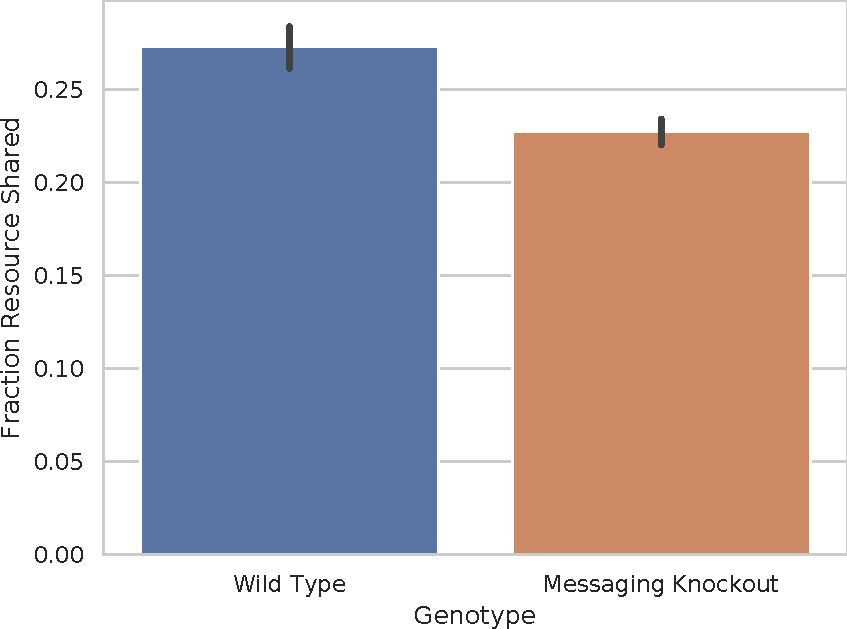
\includegraphics[width=\textwidth]{knockout/intermessaging-intergroup_border/title=sharingfraction+_data_hathash_hash=b0e9f42c3e74cf6a+_script_fullcat_hash=84ce7f4d8802dbab+_source_hash=53a2252-clean+ext=}%
\caption{Resource sharing}
\label{fig:intermessaging-intergroup_border-sharing}
\end{subfigure}
\end{minipage}%

\vspace{1ex}

\hspace*{\fill}%
\begin{minipage}[t]{0.8\columnwidth}
\centering
\vspace{0pt} % for alignment
\begin{subfigure}[b]{\textwidth}
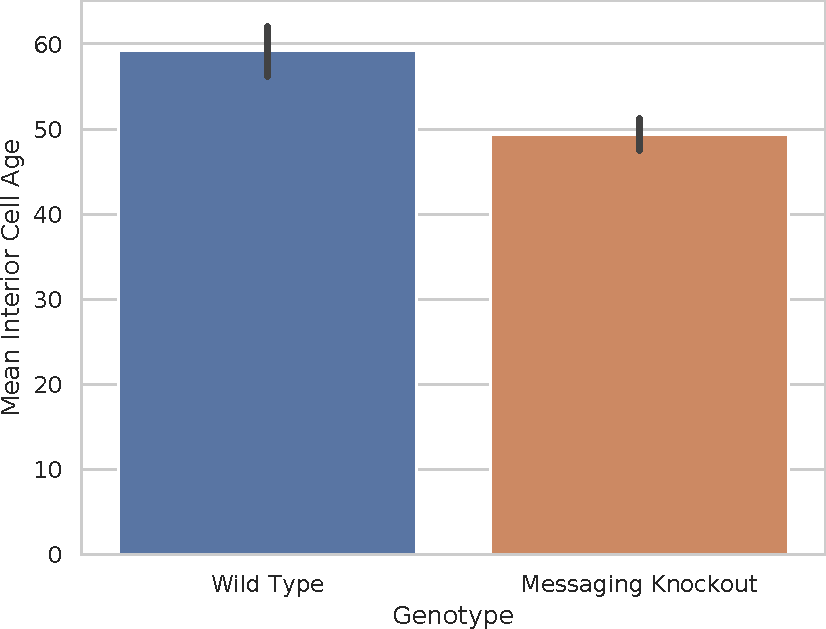
\includegraphics[width=\textwidth]{knockout/intermessaging-intergroup_border/title=cellageraw+_data_hathash_hash=ef9f5e984a40fbf6+_script_fullcat_hash=1faec38cdb6bd1de+_source_hash=53a2252-clean+ext=}%
\caption{Interior cell age}
\label{fig:intermessaging-intergroup_border-cellage}
\end{subfigure}
\end{minipage}%
\hspace*{\fill}

\end{minipage}%
\begin{minipage}[t]{\columnwidth}
\centering

\hspace*{\fill}%
\begin{minipage}[t]{0.8\columnwidth}
\centering
\vspace{0pt} % for alignment
\begin{subfigure}[b]{\textwidth}
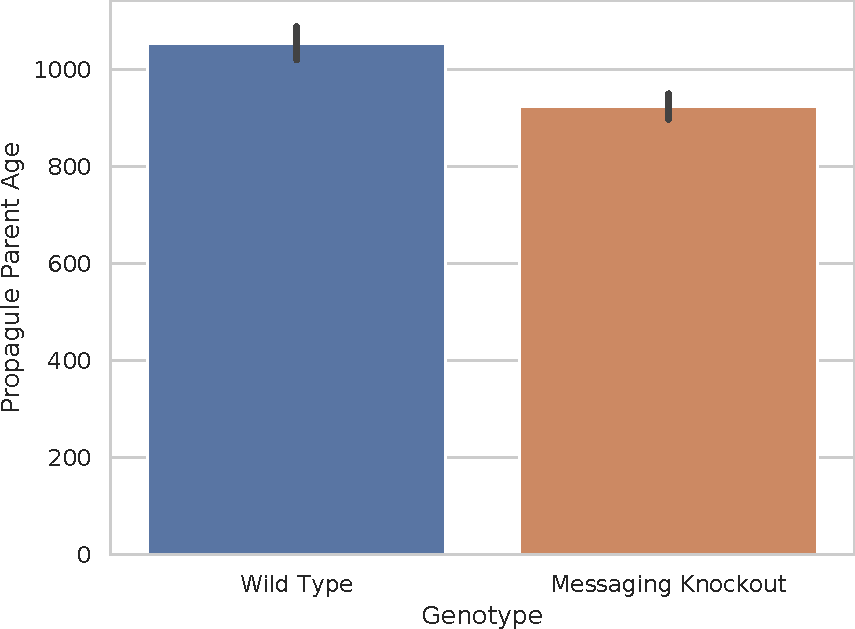
\includegraphics[width=\textwidth]{knockout/intermessaging-intergroup_border/title=parentage+_data_hathash_hash=974d02d36b7dba1a+_script_fullcat_hash=7ee3d274683ffdb2+_source_hash=53a2252-clean+ext=}%
\caption{Propagule parent age}
\label{fig:intermessaging-intergroup_border-pparentage}
\end{subfigure}
\end{minipage}%
\hspace*{\fill}

\vspace{1ex}

\hspace*{\fill}%
\begin{minipage}[t]{0.8\columnwidth}
\centering
\vspace{0pt} % for alignment
\begin{subfigure}[b]{\textwidth}
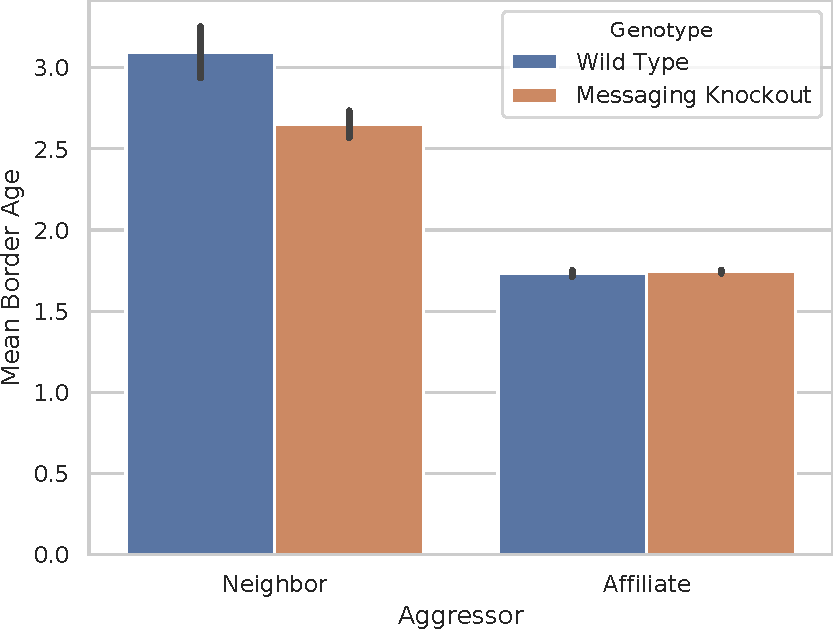
\includegraphics[width=\textwidth]{knockout/intermessaging-intergroup_border/title=comboborderage+_data_hathash_hash=8369fa84222d9217+_script_fullcat_hash=c576822d0876c8a8+_source_hash=53a2252-clean+ext=}%
\caption{Border age}
\label{fig:intermessaging-intergroup_border-borderage}
\end{subfigure}
\end{minipage}%
\hspace*{\fill}

\vspace{1ex}

\hspace*{\fill}%
\begin{minipage}[t]{0.8\columnwidth}
\centering
\vspace{0pt} % for alignment
\begin{subfigure}[b]{\textwidth}
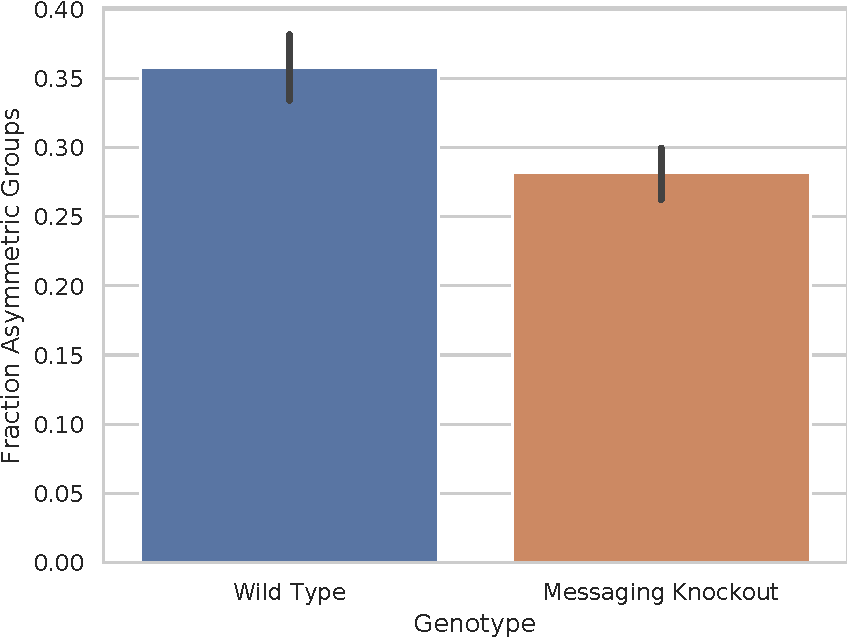
\includegraphics[width=\textwidth]{knockout/intermessaging-intergroup_border/title=metabolismasymmetry+_data_hathash_hash=3ce8f7b8474367f3+_script_fullcat_hash=0329612f3b158905+_source_hash=53a2252-clean+ext=}%
\caption{Asymmetric border metabolism}
\label{fig:intermessaging-intergroup_border-metabolism}
\end{subfigure}
\end{minipage}%
\hspace*{\fill}

\caption{
Comparison of wild type strain and corresponding intercell messaging knockout strain.
Subfigure \ref{fig:intermessaging-intergroup_border-phen} visualizes phenotypic traits in the wild type and knockout strain.
In the messaging visualization, color coding represents the volume of incoming messages.
White represents no incoming messages and the magenta to blue gradient runs from one incoming message to the maximum observed incoming message traffic.
In the resource sharing visualization, this same color coding represents the amount of incoming shared resource.
Solid black borders divide level-one same-channel signaling networks and dotted light gray borders divide level-zero same-channel signaling networks.
Subfigures \ref{fig:intermessaging-intergroup_border-sharing}, \ref{fig:intermessaging-intergroup_border-cellage}, \ref{fig:intermessaging-intergroup_border-pparentage}, \ref{fig:intermessaging-intergroup_border-borderage}, and \ref{fig:intermessaging-intergroup_border-metabolism} quantify knockout effects on various phenotypic traits.
Error bars indicate 95\% confidence.
}
\label{fig:ko-intermessaging-intergroup_border}
\end{minipage}

\end{center}
\end{figure*}


Figure \ref{fig:ko-intermessaging-sharing}

Figure \ref{fig:ko-intermessaging-intergroup_border}

\subsection{Case Studies: Apoptosis} \label{sec:apoptosis}

\begin{figure}[!htbp]
\begin{center}

\hspace*{\fill}%
\begin{minipage}[t]{0.05\columnwidth}
\vspace{0pt} % for alignment
\rotatebox{90}{Strain A}%
\end{minipage}%
\hfill
\begin{minipage}[t]{0.45\columnwidth}
\centering
\vspace{0pt} % for alignment
\adjincludegraphics[width=\textwidth, trim={{.5\width} {.5\width} {.0\width} {.0\width}}, clip]{knockout/apoptosis/wildtype/seed=1+title=channel_viz+treat=resource-even__channelsense-yes__nlev-two+update=262144+_data_hathash_hash=9b92a609c3309033+_script_fullcat_hash=7e789c981e3d0e4f+_source_hash=53a2252-clean+ext=}%
\end{minipage}%
\hfill
\begin{minipage}[t]{0.45\columnwidth}
\centering
\vspace{0pt} % for alignment
\adjincludegraphics[width=\textwidth, trim={{.5\width} {.5\width} {.0\width} {.0\width}}, clip]{knockout/apoptosis/knockout/seed=1+title=channel_viz+treat=resource-even__channelsense-yes__nlev-two+update=262144+_data_hathash_hash=900abeef45bb9133+_script_fullcat_hash=7e789c981e3d0e4f+_source_hash=53a2252-clean+ext=}%
\end{minipage}%
\hspace*{\fill}

\hspace*{\fill}%
\begin{minipage}[t]{0.05\columnwidth}
\vspace{0pt} % for alignment
\rotatebox{90}{Strain B}%
\hfill
\end{minipage}%
\hfill
\begin{minipage}[t]{0.45\columnwidth}
\centering
\vspace{0pt} % for alignment
\adjincludegraphics[width=\textwidth, trim={{.5\width} {.5\width} {.0\width} {.0\width}}, clip]{knockout/apoptosis/wildtype/seed=1+title=channel_viz+treat=resource-wave__channelsense-yes__nlev-onebig+update=8188+_data_hathash_hash=3465df2fce2dc5f4+_script_fullcat_hash=7e789c981e3d0e4f+_source_hash=53a2252-clean+ext=}
\end{minipage}%
\hfill
\begin{minipage}[t]{0.45\columnwidth}
\centering
\vspace{0pt} % for alignment
\adjincludegraphics[width=\textwidth, trim={{.5\width} {.5\width} {.0\width} {.0\width}}, clip]{knockout/apoptosis/knockout/seed=1+title=channel_viz+treat=resource-wave__channelsense-yes__nlev-onebig+update=8188+_data_hathash_hash=9c40470beee1c5b5+_script_fullcat_hash=7e789c981e3d0e4f+_source_hash=53a2252-clean+ext=}%
\end{minipage}%
\hspace*{\fill}

\vspace{1.0ex}

\hspace*{\fill}%
\begin{minipage}[t]{0.05\columnwidth}
\vspace{0pt} % for alignment
\end{minipage}%
\hfill
\begin{minipage}[t]{0.45\columnwidth}
\centering
\vspace{0pt} % for alignment
Wild Type
\end{minipage}%
\hfill
\begin{minipage}[t]{0.45\columnwidth}
\centering
\vspace{0pt} % for alignment
Apoptosis Knockout
\end{minipage}%
\hspace*{\fill}

\caption{
Comparison of wild type strains and corresponding apoptosis knockout strains.
In all visualizations, color hue denotes and black borders divide highest-level same-channel signaling networks.
In Replicate A visualizations, color saturation denotes and white borders divide level-zero same-channel signaling networks.
(Replicate B evolved under the flat treatment).
Black tiles are dead.
}
\label{fig:ko-apoptosis}
\end{center}
\end{figure}


Screening replicate evolutionary runs by apoptosis rate flagged two strains with several orders of magnitude greater activity.
In strain A, evolved under the even treatment, apoptosis accounts for 2\% of cell mortality.
In strain B, evolved under the flat treatment, 15\% of mortality is due to apoptosis.

To test the adaptive role of apoptosis in these strains, we performed competition experiments against apoptosis knockout strains, in which all apoptosis instructions were substituted for Nop instructions.
Figure \ref{fig:ko-apoptosis} compares the same-channel wild type phenotypes of these strains to their corresponding knockouts.

Apoptosis contributed significantly to fitness in both strains (strain A: $18/20$, $p < 0.001$, two-tailed exact test; strain B: $20/20$, $p < 0.001$, two-tailed exact test).
The success of strategies incorporating cell suicide is characteristic of a transition from cell-level to collective individuality.


\section{Conclusion}

Using simple organisms that evolve parameters for a set of manually-designed strategies, we have demonstrated that DISHTINY environment selects for genotypes that exhibit high-level individuality.
We observed cell-, zeroth-, and first- level individuality among evolutionary outcomes.
Specifically, we observed
\begin{enumerate}
  \item division of reproductive labor between members of the same channel (i.e. between individuals enveloped in a same-channel signaling network and those on the periphery), and
  \item cooperation between members of the same channel (i.e. pooling of resource on the same-channel signaling networks).
\end{enumerate}

Ecological trials revealed that first-level individuals outcompete zeroth- and cell-level individuals.
Interestingly, employment of strategies to combat somatic mutation through apoptosis was correlated with first-level individuality.
We observed that the magnitude of resource endowment for propagules was also correlated with first-level individuality.

Although shifts in individuality coincident with the both the zero- and the one-level signaling network were both clearly observed, the question of whether these transitions were truly hierarchical in nature is debatable.
That is, it is not clear whether zeroth-level individuality was to some extent preserved in or necessary for the emergence of first-level individuality.
Given the nature of the manually-designed strategies for resource-pooling and reproductive division of labor, first-level resource pooling and division of labor could readily leapfrog over zeroth-level resource pooling and division of labor and, in many ways, seemed to completely supersede those zero-level efforts.

We believe that this is a shortcoming of the design of organisms employed in these experiments, not the DISHTINY environment itself.
We have nevertheless clearly demonstrated that the DISHTINY environment ultimately selects for high-level individuality.
We are eager to work with more sophisticated cells capable of arbitrary computation via genetic programming in order to pursue more open-ended evolutionary experiments \cite{ofria2004avida}.
Such work will provide valuable insight into scientific questions relating to major evolutionary transitions such as the role of pre-existing phenotypic plasticity \citep{clune2007investigating, lalejini2016evolutionary}, pre-existing environmental interactions, pre-existing reproductive division of labor, and how transitions relate to increases in organizational \citep{goldsby2012task}, structural, and functional \citep{goldsby2014evolutionary} complexity.

We believe that such an approach also provides a unique opportunity to fundamentally further the ambition of the field of Artificial life with respect to open-ended evolution.
Key to this ambition is scale.
The DISHTINY environment near-trivially scales to select for an arbitrary number of hierarchical levels of individuality (not just the two hierarchical levels explored in these experiments).
Importantly, the environment is implemented in a near-completely decentralized manner.
This means that parallelization might be realized --- ultimately, perhaps on the level of the individual toroidal grid tile --- such that per-update run time can nearly remain constant whatever the area of the toroidal grid.
Parallel computing is widely exploited in evolutionary computing, where subpopulations are farmed out to individual compute nodes for for periods of isolated evolution or single genotypes are farmed out to individual compute nodes for fitness evaluation \citep{lin1994coarse, real17a}.
The DISHTINY platform presents a more fundamental parallelization potential: principled parallelization of the evolving individual phenotype at arbitrary scale (i.e. a high-level individual as a large collection of individual cells on the toroidal grid).
Such parallelization will be key to realizing evolving computational systems with scale --- and, perhaps, complexity --- approaching those of biological systems.


\section{Acknowledgements}

Thanks to members of the DEVOLAB, in particular Michael J. Wiser, for feedback on statistical methods.  This research was supported in part by the BEACON Center for the Study of Evolution in Action (NSF Cooperative Agreement No. DBI-0939454) and by Michigan State University through the computational resources provided by the Institute for Cyber-Enabled Research. Any opinions, findings, and conclusions or recommendations expressed in this material are those of the author(s) and do not necessarily reflect the views of the National Science Foundation.


\footnotesize
\bibliographystyle{apalike}
\bibliography{bibl} % replace by the name of your .bib file


\end{document}
